\chapter{Strutture succinte}
\section{Abstract data types}
Gli \textit{abstract data type} sono tipi di dati descritti dal loro comportamento: un esempio è
l'ADT \texttt{stack<T>}, il quale è dotato di alcune operazioni inerenti al tipo
stesso, chiamate \textbf{primitive}:
\begin{lstlisting}
  bool  isEmpty()
  T     top()
  void  pop()
  void  push(T)
\end{lstlisting}
Il comportamento cosa facciano i metodi si può descrivere in molti modi: si può
utilizzare un metodo discorsivo, spiegando a parole, o utilizzare un metodo
analitico:
$$
	\forall S, s.push(x).top() = x
$$
(nonostante la notazione impropria dovuta alla signatura delle funzioni);
$$
	\forall S, s.isEmpty() \implies S.push(x).pop().isEmpty()
$$
Una volta descritto un ADT è necessario implementarlo, ossia costruire effettivamente
una struttura che implementa le primitive rispettandone la descrizione. Chiaramente,
vi sono molte implementazioni diverse che soddisfano le richieste
ma hanno \textit{costi} diversi, sia in tempo che in spazio. Siamo interessati
ad alcuni ADT e relative implementazioni che utilizzano poco tempo e spazio.
Ogni ADT ha associato un concetto di \textit{taglia}, che rappresenta genericamente
la grandezza di un'istanza: nel caso dello stack, la taglia sarebbe il numero
di elementi presenti sulla pila.

\subsection{Teoria dell'informazione}
Per poter caratterizzare le implementazioni degli ADT in base allo
spazio che occupano è necessario introdurre alcuni concetti della teoria
dell'informazione, i quali discendono dai Teoremi di Shannon,
sommariamente riassumibili nel seguente teorema.

\begin{theorem}[della codifica della sorgente]
	\label{thm:shannon}
	Per codificare $v$ valori servono in media $\log_2(v)$ bit.
\end{theorem}

Per esempio, immaginiamo di dover codificare un'immagine $100\times100$ pixel
in bianco e nero. Le immagini possibili sono $2^{10000}$: per codificare
queste immagini servono in media $10000$ bit. In effetti, la
rappresentazione banale che rappresenta ogni pixel, utilizza esattamente
$10000$ bit e non potrebbe usarne di meno! Usandone, per esempio, solo
$9000$, alcune immagini diverse avrebbero la stessa rappresentazione.

Questo teorema vale anche per rappresentazioni di dimensione
variabile, ossia vale anche per codifiche: si supponga di avere un
algoritmo in grado di comprimere tre immagini ognuna in $100$ bit.
La conseguenza di questo teorema è che ci saranno delle altre immagini che
utlizzeranno più di $10000$ bit, in modo che la media rimanga $10000$.

In generale, dati $v$ valori rappresentabili con $x_1, x_2, \cdots, x_v$ bit
rispettivamente; il Teorema afferma che
$$
	\frac{\sum_{i} x_i}{v} \geq \log_2(v)
$$
%(
di così e che esiste un sistema di compressione che riesce a rappresentare
in realtà il \cref{thm:shannon} dice di più, ossia che non si può fare meglio
i $v$ valori utilizzando un numero di bit medio tra $[\log_2(v), 1 + \log_2(v))$,
assumendo che tutti i $v$ valori siano equiprobabili\footnote{
	\cite{shannon_1948} è il lavoro di C. Shannon che ha dato vita al campo della
	teoria dell'informazione; un approccio più moderno è \cite{cover_2006}. }.
%]

Ci confronteremo spesso con questo \textbf{information-theoretical lower bound}:
immaginiamo tutte le possibili istanze $v_i$ di ADT di taglia $i$;
per esempio, uno stack con valori in $\{0, 1, \cdots, 9\}$;
lo stack di taglia $0$ è lo stack vuoto, gli stack
di taglia $1$ sono le $10$ istanze stack che contengono solo $1$, solo $2$, e così via,
mentre gli stack di taglia $2$ sono $10^2$; in generale uno stack
di taglia $n$ ha $10^n$ valori. Il Teorema afferma che in media servono
$\log_2{10^n} = n \log_2(10) \approx 4n$ bit per rappresentare uno stack
con valori in $\{0, 1, \cdots, 9\}$: sappiamo quindi che
\textit{nessuna implementazione} può utilizzare, in media, meno di
$Z_n =n \log_2(10)$ bit, l'information-theoretical lower bound per
rappresentare stack di taglia $n$ con valori in $\{0, 1, \cdots, 9\}$.

Ipotizziamo di avere una struttura che utilizza in media $D_n \geq Z_n$ bit:
esiste un tradeoff tra quanto \textit{compatta} è la struttura e quanto
tempo è necessario per eseguire le funzioni primitive.
Esistono sistemi di compressione che ignorano completamente il problema:
ad esempio, comprimendo un oggetto con l'algoritmo \texttt{tz2}, non si può
utilizzare l'oggetto compresso come la sua rappresentazione non compressa
per eseguire le primitive su di esso! Noi siamo interessati a strutture
compresse - rappresentano i dati in maniera efficiente rispetto allo spazio -
e con primitive efficienti tanto quanto un'implementazione non compressa.

Definiamo quindi delle classificazioni delle implementazioni in base al rapporto
tra l'effettivo utilizzo di spazio (in media) e l'indice $Z_n$:
un'implementazione dell'ADT è chiamata \textbf{implicita} se occupa un numero
di bit $D_n = Z_n + O(1)$, \textbf{succinta} se occupa un numero di bit
$D_n = Z_n + o(Z_n)$ e \textbf{compatta} se $D_n = O(Z_n)$; tutto questo sempre
notando che le primitive devono essere efficienti tanto quanto quelle definite
su strutture non compresse.

\section{Strutture di rango e selezione}
Questi ADT sono definiti da un vettore $\mathbb{b} \in 2^n$ con due primitive:
$$
	\mathbf{rank}_b = \mathbb{N} \rightarrow \mathbb{N}
$$
$$
	\mathbf{select}_b= \mathbb{N} \rightarrow \mathbb{N}
$$
tali che:
$$
	\forall p \leq n ~~ \mathbf{rank}_b(p) = |\{i | i < p \land b_i = 1\}|
$$
$$
	\forall k \leq n ~~ \mathbf{select}_b(k) =\max \{p | \mathbf{rank}_b(p) \leq k\}
$$
Quindi, per esempio, per un $\mathbf{b} = [0 1 1 0 1 0 1]$ si hanno due
tabelle di rank e select come in \cref{table:rank_sel}.

\begin{table}[ht]
	\centering

	\begin{subtable}{0.45\textwidth}
		\centering
		\begin{tabular}{c|c}
			$p$ & $\mathbf{rank}_b(p)$ \\ \hline
			0   & 0                    \\
			1   & 0                    \\
			2   & 1                    \\
			3   & 2                    \\
			4   & 2                    \\
			5   & 3                    \\
			6   & 3                    \\
			7   & 4
		\end{tabular}
		\caption{$\mathbf{rank}_b(p)$}
	\end{subtable}
	\begin{subtable}{0.45\textwidth}
		\centering
		\begin{tabular}{c|c}
			$k$      & $\mathbf{select}_b(p)$ \\ \hline
			0        & 1                      \\
			1        & 2                      \\
			2        & 3                      \\
			3        & 6                      \\
			4        & 7                      \\
			5        & 7                      \\
			$\cdots$ & 7                      \\
		\end{tabular}
		\caption{$\mathbf{select}_b(p)$}
	\end{subtable}
	\caption{Tabelle per $\mathbf{b}$.}
	\label{table:rank_sel}
\end{table}
Rank e select sono funzioni inverse in un senso molto stretto, ciò vale che
$$
	\forall k ~~ \mathbf{rank}_b(\mathbf{select}_b(k)) = k
$$
mentre l'inverso, ossia applicare select a rank, si ottiene una proprietà
diversa:
$$
	\forall p ~~ \mathbf{select}_b(\mathbf{rank}_b(p)) \geq p
$$
proprio grazie a quest'ultima proprietà è possibile dedurre la struttura sottostante,
nel senso che è possibile capire dove siano gli $0$ e gli $1$ in $\mathbf{b}$.

\subsection{Strutture di Jacobson per il rango}
\subsubsection{Four-russians trick}
L'implementazione dell'ADT rank di Jacobson
utilizza il ``four-russians trick''. Si immagini di
voler rappresentare una matrice binaria: un modo per farlo potrebbe essere
dividere la matrice in blocchi chiamati \textit{piastrelle} ed enumerare
le possibili piastrelle. Chiaramente, se nella matrice appare ogni possibile
combinazione di piastrella, il guadagno del trucco sarà nullo.
Se, invece, la matrice è molto ripetitiva, le piastrelle possibili da ricordare saranno
poche e basterà utilizzare il numero associato alla piastrella per rappresentare
l'intera matrice. Un esempio è in \cref{fig:frtrick}.

% disegno.. 19-11-2021 ... 
\begin{figure}[ht]
	\centering
	\begin{subfigure}{0.32\textwidth}
		\centering
		\tikzset{every picture/.style={line width=0.75pt}} %set default line width to 0.75pt        

		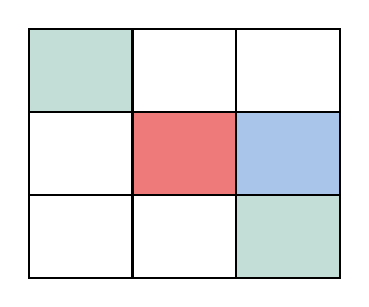
\begin{tikzpicture}[x=0.75pt,y=0.75pt,yscale=-1,xscale=1]
			%uncomment if require: \path (0,300); %set diagram left start at 0, and has height of 300

			%Shape: Rectangle [id:dp005749332004390428] 
			\draw  [fill={rgb, 255:red, 195; green, 222; blue, 215 }  ,fill opacity=1 ] (10,30) -- (60,30) -- (60,70) -- (10,70) -- cycle ;
			%Shape: Rectangle [id:dp7752907448209945] 
			\draw   (60,30) -- (110,30) -- (110,70) -- (60,70) -- cycle ;
			%Shape: Rectangle [id:dp6434156098479539] 
			\draw   (110,30) -- (160,30) -- (160,70) -- (110,70) -- cycle ;
			%Shape: Rectangle [id:dp6511151383263759] 
			\draw   (10,70) -- (60,70) -- (60,110) -- (10,110) -- cycle ;
			%Shape: Rectangle [id:dp12594297400828225] 
			\draw  [color={rgb, 255:red, 0; green, 0; blue, 0 }  ,draw opacity=1 ][fill={rgb, 255:red, 239; green, 122; blue, 122 }  ,fill opacity=1 ] (60,70) -- (110,70) -- (110,110) -- (60,110) -- cycle ;
			%Shape: Rectangle [id:dp07170680173867716] 
			\draw  [fill={rgb, 255:red, 169; green, 198; blue, 234 }  ,fill opacity=1 ] (110,70) -- (160,70) -- (160,110) -- (110,110) -- cycle ;
			%Shape: Rectangle [id:dp016792670255308284] 
			\draw   (10,110) -- (60,110) -- (60,150) -- (10,150) -- cycle ;
			%Shape: Rectangle [id:dp40735665999968684] 
			\draw   (60,110) -- (110,110) -- (110,150) -- (60,150) -- cycle ;
			%Shape: Rectangle [id:dp5192196869257351] 
			\draw  [fill={rgb, 255:red, 195; green, 222; blue, 215 }  ,fill opacity=1 ] (110,110) -- (160,110) -- (160,150) -- (110,150) -- cycle ;
		\end{tikzpicture}
		\caption{Tabella iniziale. Ogni riquadro contiene $5$ bit.}
	\end{subfigure}
	\begin{subfigure}{0.32\textwidth}
		\centering

		\tikzset{every picture/.style={line width=0.75pt}} %set default line width to 0.75pt        

		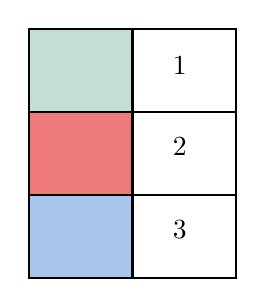
\begin{tikzpicture}[x=0.75pt,y=0.75pt,yscale=-1,xscale=1]
			%uncomment if require: \path (0,300); %set diagram left start at 0, and has height of 300

			%Shape: Rectangle [id:dp7804092113436614] 
			\draw  [fill={rgb, 255:red, 195; green, 222; blue, 215 }  ,fill opacity=1 ] (200,50) -- (250,50) -- (250,90) -- (200,90) -- cycle ;
			%Shape: Rectangle [id:dp023528268951144793] 
			\draw  [fill={rgb, 255:red, 239; green, 122; blue, 122 }  ,fill opacity=1 ] (200,90) -- (250,90) -- (250,130) -- (200,130) -- cycle ;
			%Shape: Rectangle [id:dp43332731525643986] 
			\draw  [fill={rgb, 255:red, 169; green, 198; blue, 234 }  ,fill opacity=1 ] (200,130) -- (250,130) -- (250,170) -- (200,170) -- cycle ;
			%Shape: Rectangle [id:dp31985072077933197] 
			\draw   (250,50) -- (300,50) -- (300,90) -- (250,90) -- cycle ;

			%Shape: Rectangle [id:dp6876058724781219] 
			\draw   (250,90) -- (300,90) -- (300,130) -- (250,130) -- cycle ;

			%Shape: Rectangle [id:dp9303810523957489] 
			\draw   (250,130) -- (300,130) -- (300,170) -- (250,170) -- cycle ;

			% Text Node
			\draw (268,141) node [anchor=north west][inner sep=0.75pt]   [align=left] {3};
			% Text Node
			\draw (268,101) node [anchor=north west][inner sep=0.75pt]   [align=left] {2};
			% Text Node
			\draw (268,62) node [anchor=north west][inner sep=0.75pt]   [align=left] {1};
		\end{tikzpicture}
		\caption{Enumerazione di sottomatrici.}
	\end{subfigure}
	\begin{subfigure}{0.32\textwidth}
		\centering
		\tikzset{every picture/.style={line width=0.75pt}} %set default line width to 0.75pt        

		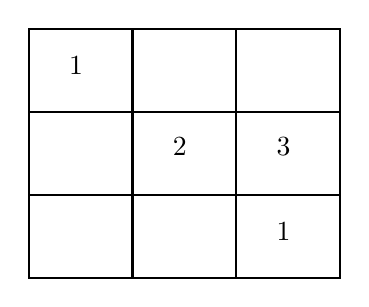
\begin{tikzpicture}[x=0.75pt,y=0.75pt,yscale=-1,xscale=1]
			%uncomment if require: \path (0,300); %set diagram left start at 0, and has height of 300

			%Shape: Rectangle [id:dp021688033849312616] 
			\draw   (295,78) -- (345,78) -- (345,118) -- (295,118) -- cycle ;
			%Shape: Rectangle [id:dp6593678571435228] 
			\draw   (345,78) -- (395,78) -- (395,118) -- (345,118) -- cycle ;
			%Shape: Rectangle [id:dp05373113383793526] 
			\draw  [fill={rgb, 255:red, 195; green, 222; blue, 215 }  ,fill opacity=0 ] (245,118) -- (295,118) -- (295,158) -- (245,158) -- cycle ;
			%Shape: Rectangle [id:dp881184835248234] 
			\draw  [fill={rgb, 255:red, 195; green, 222; blue, 215 }  ,fill opacity=0 ] (245,158) -- (295,158) -- (295,198) -- (245,198) -- cycle ;
			%Shape: Rectangle [id:dp40942537357979314] 
			\draw   (295,158) -- (345,158) -- (345,198) -- (295,198) -- cycle ;
			%Shape: Rectangle [id:dp4268873556029348] 
			\draw   (245,78) -- (295,78) -- (295,118) -- (245,118) -- cycle ;

			%Shape: Rectangle [id:dp9673334799284516] 
			\draw   (345,158) -- (395,158) -- (395,198) -- (345,198) -- cycle ;

			%Shape: Rectangle [id:dp06125848702433001] 
			\draw   (295,118) -- (345,118) -- (345,158) -- (295,158) -- cycle ;

			%Shape: Rectangle [id:dp6270788142678815] 
			\draw   (345,118) -- (395,118) -- (395,158) -- (345,158) -- cycle ;


			% Text Node
			\draw (363,129) node [anchor=north west][inner sep=0.75pt]   [align=left] {3};
			% Text Node
			\draw (313,129) node [anchor=north west][inner sep=0.75pt]   [align=left] {2};
			% Text Node
			\draw (363,170) node [anchor=north west][inner sep=0.75pt]   [align=left] {1};
			% Text Node
			\draw (263,90) node [anchor=north west][inner sep=0.75pt]   [align=left] {1};


		\end{tikzpicture}
		\caption{Matrice risultante dopo l'applicazione del \textit{four-russians trick}.}
	\end{subfigure}
	\caption{}
	\label{fig:frtrick}
\end{figure}

% lezione 17 - 24-11-2021
\subsubsection{Implementazione}
Il vettore $\mathbf{b}$  di $n$ bit viene quindi diviso in blocchi della
stessa lunghezza, chiamati \textit{superblocchi}, di lunghezza
$\log_2(n)^2$. Ogni superblocco viene
diviso a sua volta in blocchi più piccoli, di lunghezza $\frac{1}{2} \log_2(n)$,
come rappresentato in \cref{fig:jrank}.
\begin{figure}[ht]
	\centering
	\tikzset{every picture/.style={line width=0.75pt}} %set default line width to 0.75pt        

	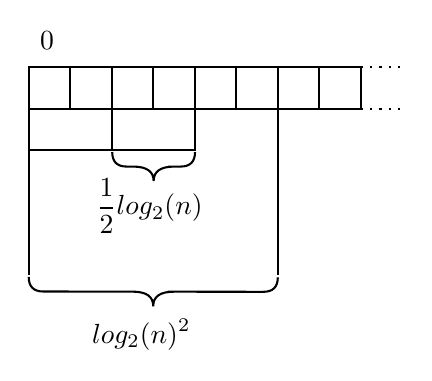
\begin{tikzpicture}[x=0.75pt,y=0.75pt,yscale=-1,xscale=1]
		%uncomment if require: \path (0,300); %set diagram left start at 0, and has height of 300

		%Shape: Brace [id:dp6738156163571107] 
		\draw   (150,231) .. controls (149.99,235.67) and (152.32,238) .. (156.99,238.01) -- (199.99,238.07) .. controls (206.66,238.08) and (209.99,240.41) .. (209.98,245.08) .. controls (209.99,240.41) and (213.32,238.09) .. (219.99,238.1)(216.99,238.09) -- (262.99,238.16) .. controls (267.66,238.17) and (269.99,235.84) .. (270,231.17) ;
		%Straight Lines [id:da0175742846479654] 
		\draw    (150,150) -- (150,230) ;
		%Straight Lines [id:da9565831392918982] 
		\draw    (270,150) -- (270,230) ;
		%Shape: Rectangle [id:dp2322340296066201] 
		\draw   (150,130) -- (170,130) -- (170,150) -- (150,150) -- cycle ;
		%Shape: Rectangle [id:dp44447847120593675] 
		\draw   (170,130) -- (190,130) -- (190,150) -- (170,150) -- cycle ;
		%Shape: Rectangle [id:dp11830121656354553] 
		\draw   (190,130) -- (210,130) -- (210,150) -- (190,150) -- cycle ;
		%Shape: Rectangle [id:dp03816859758995417] 
		\draw   (210,130) -- (230,130) -- (230,150) -- (210,150) -- cycle ;
		%Shape: Rectangle [id:dp9408927207358553] 
		\draw   (230,130) -- (250,130) -- (250,150) -- (230,150) -- cycle ;
		%Shape: Rectangle [id:dp9557419136965325] 
		\draw   (250,130) -- (270,130) -- (270,150) -- (250,150) -- cycle ;
		%Shape: Rectangle [id:dp7039774887247845] 
		\draw   (270,130) -- (290,130) -- (290,150) -- (270,150) -- cycle ;
		%Shape: Rectangle [id:dp3777415956586846] 
		\draw   (290,130) -- (310,130) -- (310,150) -- (290,150) -- cycle ;
		%Shape: Rectangle [id:dp35581942359165963] 
		\draw   (150,150) -- (190,150) -- (190,170) -- (150,170) -- cycle ;
		%Shape: Rectangle [id:dp047912414707197204] 
		\draw   (190,150) -- (230,150) -- (230,170) -- (190,170) -- cycle ;
		%Shape: Brace [id:dp6450376307720747] 
		\draw   (190.22,170.82) .. controls (190.22,175.49) and (192.55,177.82) .. (197.22,177.82) -- (200.17,177.82) .. controls (206.84,177.82) and (210.17,180.15) .. (210.17,184.82) .. controls (210.17,180.15) and (213.5,177.82) .. (220.17,177.82)(217.17,177.82) -- (223.11,177.82) .. controls (227.78,177.82) and (230.11,175.49) .. (230.11,170.82) ;
		%Straight Lines [id:da007337321639370731] 
		\draw  [dash pattern={on 0.84pt off 2.51pt}]  (310,130) -- (330,130) ;
		%Straight Lines [id:da4459939594214508] 
		\draw  [dash pattern={on 0.84pt off 2.51pt}]  (310,150) -- (330,150) ;

		% Text Node
		\draw (179,250) node [anchor=north west][inner sep=0.75pt]   [align=left] {$\displaystyle log_{2}( n)^{2}$};
		% Text Node
		\draw (181,182) node [anchor=north west][inner sep=0.75pt]   [align=left] {$\displaystyle \frac{1}{2} log_{2}( n)$};
		% Text Node
		\draw (154,111.4) node [anchor=north west][inner sep=0.75pt]    {$0$};


	\end{tikzpicture}
	\caption{Divisione di $\textbf{b}$ in superblocchi e blocchi.}
	\label{fig:jrank}
\end{figure}
Per esempio, se $n = 256$, i superblocchi avranno lunghezza
$\log_2(256)^2 = 8^2 = 64$ bit e saranno $256/64 = 4$, mentre i
blocchi interni saranno $\frac{1}{2}\log_2(256) = \frac{1}{2}8 = 4$ bit e saranno
$64/4 = 16$ per superblocco, $16*4 = 64$ in totale.
In questo esempio, i possibili blocchi sono $2^4 = 16$ e, in generale,
siccome i blocchi hanno lunghezza $\frac{1}{2} \log_2(n)$, sono
$$
	2^{\frac{1}{2}\log_2(n)} = (2^{\log_2(n)})^{\frac{1}{2}} =  \sqrt{n}
$$
Se volessimo memorizzare la funzione di rank per un singolo blocco,
costruiremmo una tabella di $\frac{1}{2}\log_2(n)$ righe e per ognuna
di queste bisognerebbe salvare il numero di $1$ presenti nel blocco fino a quel punto,
utilizzando per ogni rank uno spazio $\log_2(\frac{1}{2}\log_2(n))$. Interamente, quindi,
la tabella di rank per un singolo blocco occupa spazio
$$
	\frac{1}{2}\log_2(n) \cdot \log_2(\frac{1}{2}\log_2(n)) \text{ bit}
$$
e, volendo memorizzare la tabella per ogni tipo di blocco, si consuma uno spazio
$$
	2^{\frac{1}{2}\log_2(n)} \cdot \frac{1}{2}\log_2(n) \cdot \log_2(\frac{1}{2}\log_2(n)) = \sqrt{n} \cdot \frac{1}{2}\log_2(n) \cdot \log_2(\frac{1}{2}\log_2(n))
	\leq \sqrt{n} \frac{1}{2}\log_2(n) \cdot \log_2(\log_2(n)) = o(n) \text{ bit}
$$
che significa che si può definire una tabella che enumera i tipi di blocco e per ognuno di
essi, come mostrato nella \cref{table:example_rank_block4}.

\begin{table}[!ht]
	\centering
	\begin{tabular}{|c|c|c|c|c|c|c|}
		\hline
		\multirow{2}{*}{$0000$} & $p$                & $0$ & $1$ & $2$ & $3$ & $4$ \\ \cline{2-7}
		                        & $\mathbf{rank}(p)$ & $0$ & $0$ & $0$ & $0$ & $0$ \\ \hline
		\multirow{2}{*}{$0001$} & $p$                & $0$ & $1$ & $2$ & $3$ & $4$ \\ \cline{2-7}
		                        & $\mathbf{rank}(p)$ & $0$ & $0$ & $0$ & $0$ & $1$ \\ \hline
		$\cdots$                &                    &     &     &     &     &     \\ \hline
		\multirow{2}{*}{$1111$} & $p$                & $0$ & $1$ & $2$ & $3$ & $4$ \\ \cline{2-7}
		                        & $\mathbf{rank}(p)$ & $0$ & $1$ & $2$ & $3$ & $4$ \\ \hline
	\end{tabular}
	\caption{Rank per ogni possibile blocco di lunghezza $4$.}
	\label{table:example_rank_block4}
\end{table}

Tutta questa struttura, benché sembra molto grande, è in realtà memorizzabile in $o(n)$, ossia
in una quantità di spazio che cresce meno rapidamente rispetto a $n$.
La prima idea è memorizzare queste strutture di rank per i blocchi. Dopo di che, per ogni superblocco
si memorizzano gli $1$ prima del superblocco, ossia per ogni superblocco $i$ si definisce
$$
	S_i = \mathbf{rank}(i[0])
$$
come rappresentato nella \cref{fig:superblock_i}.
\begin{figure}
	\centering
	\tikzset{every picture/.style={line width=0.75pt}} %set default line width to 0.75pt        
	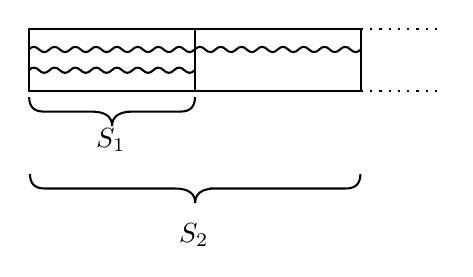
\begin{tikzpicture}[x=0.75pt,y=0.75pt,yscale=-1,xscale=1]
		%uncomment if require: \path (0,300); %set diagram left start at 0, and has height of 300

		%Shape: Brace [id:dp6450376307720747] 
		\draw   (150.22,152.93) .. controls (150.22,157.6) and (152.55,159.93) .. (157.22,159.93) -- (180.17,159.93) .. controls (186.84,159.93) and (190.17,162.26) .. (190.17,166.93) .. controls (190.17,162.26) and (193.5,159.93) .. (200.17,159.93)(197.17,159.93) -- (223.11,159.93) .. controls (227.78,159.93) and (230.11,157.6) .. (230.11,152.93) ;
		%Shape: Brace [id:dp6867457932235534] 
		\draw   (150.62,189.98) .. controls (150.62,194.65) and (152.95,196.98) .. (157.62,196.98) -- (220.21,196.98) .. controls (226.88,196.98) and (230.21,199.31) .. (230.21,203.98) .. controls (230.21,199.31) and (233.54,196.98) .. (240.21,196.98)(237.21,196.98) -- (302.8,196.98) .. controls (307.47,196.98) and (309.8,194.65) .. (309.8,189.98) ;
		%Shape: Rectangle [id:dp04043578965235095] 
		\draw   (150,120) -- (310,120) -- (310,150) -- (150,150) -- cycle ;
		%Straight Lines [id:da7948124479327557] 
		\draw    (230,120) -- (230,150) ;
		%Straight Lines [id:da6507675221013395] 
		\draw    (150,140) .. controls (151.67,138.33) and (153.33,138.33) .. (155,140) .. controls (156.67,141.67) and (158.33,141.67) .. (160,140) .. controls (161.67,138.33) and (163.33,138.33) .. (165,140) .. controls (166.67,141.67) and (168.33,141.67) .. (170,140) .. controls (171.67,138.33) and (173.33,138.33) .. (175,140) .. controls (176.67,141.67) and (178.33,141.67) .. (180,140) .. controls (181.67,138.33) and (183.33,138.33) .. (185,140) .. controls (186.67,141.67) and (188.33,141.67) .. (190,140) .. controls (191.67,138.33) and (193.33,138.33) .. (195,140) .. controls (196.67,141.67) and (198.33,141.67) .. (200,140) .. controls (201.67,138.33) and (203.33,138.33) .. (205,140) .. controls (206.67,141.67) and (208.33,141.67) .. (210,140) .. controls (211.67,138.33) and (213.33,138.33) .. (215,140) .. controls (216.67,141.67) and (218.33,141.67) .. (220,140) .. controls (221.67,138.33) and (223.33,138.33) .. (225,140) .. controls (226.67,141.67) and (228.33,141.67) .. (230,140) -- (230,140) ;
		%Straight Lines [id:da816948397241291] 
		\draw    (150,130) .. controls (151.67,128.33) and (153.33,128.33) .. (155,130) .. controls (156.67,131.67) and (158.33,131.67) .. (160,130) .. controls (161.67,128.33) and (163.33,128.33) .. (165,130) .. controls (166.67,131.67) and (168.33,131.67) .. (170,130) .. controls (171.67,128.33) and (173.33,128.33) .. (175,130) .. controls (176.67,131.67) and (178.33,131.67) .. (180,130) .. controls (181.67,128.33) and (183.33,128.33) .. (185,130) .. controls (186.67,131.67) and (188.33,131.67) .. (190,130) .. controls (191.67,128.33) and (193.33,128.33) .. (195,130) .. controls (196.67,131.67) and (198.33,131.67) .. (200,130) .. controls (201.67,128.33) and (203.33,128.33) .. (205,130) .. controls (206.67,131.67) and (208.33,131.67) .. (210,130) .. controls (211.67,128.33) and (213.33,128.33) .. (215,130) .. controls (216.67,131.67) and (218.33,131.67) .. (220,130) .. controls (221.67,128.33) and (223.33,128.33) .. (225,130) .. controls (226.67,131.67) and (228.33,131.67) .. (230,130) .. controls (231.67,128.33) and (233.33,128.33) .. (235,130) .. controls (236.67,131.67) and (238.33,131.67) .. (240,130) .. controls (241.67,128.33) and (243.33,128.33) .. (245,130) .. controls (246.67,131.67) and (248.33,131.67) .. (250,130) .. controls (251.67,128.33) and (253.33,128.33) .. (255,130) .. controls (256.67,131.67) and (258.33,131.67) .. (260,130) .. controls (261.67,128.33) and (263.33,128.33) .. (265,130) .. controls (266.67,131.67) and (268.33,131.67) .. (270,130) .. controls (271.67,128.33) and (273.33,128.33) .. (275,130) .. controls (276.67,131.67) and (278.33,131.67) .. (280,130) .. controls (281.67,128.33) and (283.33,128.33) .. (285,130) .. controls (286.67,131.67) and (288.33,131.67) .. (290,130) .. controls (291.67,128.33) and (293.33,128.33) .. (295,130) .. controls (296.67,131.67) and (298.33,131.67) .. (300,130) .. controls (301.67,128.33) and (303.33,128.33) .. (305,130) .. controls (306.67,131.67) and (308.33,131.67) .. (310,130) -- (310,130) ;
		%Straight Lines [id:da005001855200690519] 
		\draw  [dash pattern={on 0.84pt off 2.51pt}]  (310,120) -- (350,120) ;
		%Straight Lines [id:da8158288414744241] 
		\draw  [dash pattern={on 0.84pt off 2.51pt}]  (310,150) -- (350,150) ;

		% Text Node
		\draw (181,166.4) node [anchor=north west][inner sep=0.75pt]    {$S_{1}$};
		% Text Node
		\draw (221,212.4) node [anchor=north west][inner sep=0.75pt]    {$S_{2}$};
	\end{tikzpicture}
	\caption{$S_2$ è il numero di $1$ presenti in $\mathbf{b}$ `sotto' la traccia più lunga, mentre $S_1$
		è il numero di $1$ sotto quella più corta. Va notato che $S_0 = 0$ benché non sia
		mostrato nella figura.}
	\label{fig:superblock_i}
\end{figure}
Per ogni blocco $l$ afferente al superblocco $i$ si definisce
$$
	B_l = \mathbf{rank}(l[0]) - S_i
$$
come rappresentato nella \cref{fig:block_i}.
\begin{figure}
	\centering



	\tikzset{every picture/.style={line width=0.75pt}} %set default line width to 0.75pt        

	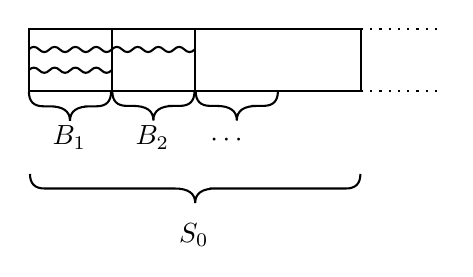
\begin{tikzpicture}[x=0.75pt,y=0.75pt,yscale=-1,xscale=1]
		%uncomment if require: \path (0,300); %set diagram left start at 0, and has height of 300

		%Shape: Brace [id:dp6867457932235534] 
		\draw   (150.62,189.98) .. controls (150.62,194.65) and (152.95,196.98) .. (157.62,196.98) -- (220.21,196.98) .. controls (226.88,196.98) and (230.21,199.31) .. (230.21,203.98) .. controls (230.21,199.31) and (233.54,196.98) .. (240.21,196.98)(237.21,196.98) -- (302.8,196.98) .. controls (307.47,196.98) and (309.8,194.65) .. (309.8,189.98) ;
		%Shape: Rectangle [id:dp04043578965235095] 
		\draw   (150,120) -- (310,120) -- (310,150) -- (150,150) -- cycle ;
		%Straight Lines [id:da005001855200690519] 
		\draw  [dash pattern={on 0.84pt off 2.51pt}]  (310,120) -- (350,120) ;
		%Straight Lines [id:da8158288414744241] 
		\draw  [dash pattern={on 0.84pt off 2.51pt}]  (310,150) -- (350,150) ;
		%Shape: Brace [id:dp13835137879055492] 
		\draw   (150.09,150.38) .. controls (150.09,155.05) and (152.42,157.38) .. (157.09,157.38) -- (159.88,157.38) .. controls (166.55,157.38) and (169.88,159.71) .. (169.88,164.38) .. controls (169.88,159.71) and (173.21,157.38) .. (179.88,157.38)(176.88,157.38) -- (182.67,157.38) .. controls (187.34,157.38) and (189.67,155.05) .. (189.67,150.38) ;
		%Shape: Brace [id:dp46357313811514655] 
		\draw   (190.28,150.18) .. controls (190.28,154.85) and (192.61,157.18) .. (197.28,157.18) -- (200.07,157.18) .. controls (206.74,157.18) and (210.07,159.51) .. (210.07,164.18) .. controls (210.07,159.51) and (213.4,157.18) .. (220.07,157.18)(217.07,157.18) -- (222.86,157.18) .. controls (227.53,157.18) and (229.86,154.85) .. (229.86,150.18) ;
		%Shape: Brace [id:dp8791020491294269] 
		\draw   (230.47,150.18) .. controls (230.47,154.85) and (232.8,157.18) .. (237.47,157.18) -- (240.26,157.18) .. controls (246.93,157.18) and (250.26,159.51) .. (250.26,164.18) .. controls (250.26,159.51) and (253.59,157.18) .. (260.26,157.18)(257.26,157.18) -- (263.05,157.18) .. controls (267.72,157.18) and (270.05,154.85) .. (270.05,150.18) ;
		%Straight Lines [id:da2991531768387089] 
		\draw    (190,120) -- (190,150) ;
		%Straight Lines [id:da7604970738017156] 
		\draw    (230,120) -- (230,150) ;
		%Straight Lines [id:da9790584425339227] 
		\draw    (150,140) .. controls (151.67,138.33) and (153.33,138.33) .. (155,140) .. controls (156.67,141.67) and (158.33,141.67) .. (160,140) .. controls (161.67,138.33) and (163.33,138.33) .. (165,140) .. controls (166.67,141.67) and (168.33,141.67) .. (170,140) .. controls (171.67,138.33) and (173.33,138.33) .. (175,140) .. controls (176.67,141.67) and (178.33,141.67) .. (180,140) .. controls (181.67,138.33) and (183.33,138.33) .. (185,140) .. controls (186.67,141.67) and (188.33,141.67) .. (190,140) -- (190,140) ;
		%Straight Lines [id:da7640613174865398] 
		\draw    (150,130) .. controls (151.67,128.33) and (153.33,128.33) .. (155,130) .. controls (156.67,131.67) and (158.33,131.67) .. (160,130) .. controls (161.67,128.33) and (163.33,128.33) .. (165,130) .. controls (166.67,131.67) and (168.33,131.67) .. (170,130) .. controls (171.67,128.33) and (173.33,128.33) .. (175,130) .. controls (176.67,131.67) and (178.33,131.67) .. (180,130) .. controls (181.67,128.33) and (183.33,128.33) .. (185,130) .. controls (186.67,131.67) and (188.33,131.67) .. (190,130) .. controls (191.67,128.33) and (193.33,128.33) .. (195,130) .. controls (196.67,131.67) and (198.33,131.67) .. (200,130) .. controls (201.67,128.33) and (203.33,128.33) .. (205,130) .. controls (206.67,131.67) and (208.33,131.67) .. (210,130) .. controls (211.67,128.33) and (213.33,128.33) .. (215,130) .. controls (216.67,131.67) and (218.33,131.67) .. (220,130) .. controls (221.67,128.33) and (223.33,128.33) .. (225,130) .. controls (226.67,131.67) and (228.33,131.67) .. (230,130) -- (230,130) ;

		% Text Node
		\draw (221,212.4) node [anchor=north west][inner sep=0.75pt]    {$S_{0}$};
		% Text Node
		\draw (160,165.4) node [anchor=north west][inner sep=0.75pt]    {$B_{1}$};
		% Text Node
		\draw (200,165.4) node [anchor=north west][inner sep=0.75pt]    {$B_{2}$};
		% Text Node
		\draw (236,169.4) node [anchor=north west][inner sep=0.75pt]    {$\cdots $};
	\end{tikzpicture}
	\caption{$B_2$ è il numero di $1$ presenti in $\mathbf{b}$ `sotto' la traccia più lunga, mentre $B_1$
		è il numero di $1$ sotto quella più corta. Va notato che $B_0$, in questo frangente, è $0$,
		poiché $S_0$ è il primo superblocco di $\mathbf{b}$.}
	\label{fig:block_i}
\end{figure}

\noindent
Quindi, gli $S_i$ sono tanti quanti sono i superblocchi, ossia $\frac{n}{log_2(n)^2}$ e occupano spazio
$$
	\frac{n}{\log_2(n)^2} \underbrace{\log_2(n)}_{\text{spazio di un } S_I} = \frac{n}{\log_2(n)} = o(n) \text{ bit}
$$
mentre i $B_l$ sono tanti quanti sono i blocchi, ossia $\frac{n}{\frac{1}{2}\log_2(n)}$ e occupano spazio
$$
	\frac{n}{\frac{1}{2}\log_2(n)} \underbrace{\log_2(\log_2(n)^2)}_{\text{al massimo}} =
	\frac{2n}{\log_2(n)} 2 \log_2(\log_2(n)) = o(n) \text{ bit}
$$
Se si vuole conoscere il rango di uno specifico bit in un blocco bisogna
recuperare $S_i$ e $B_i$ e calcolare il quale sia effettivamente il rango, che
è stato memorizzato in una tabella $Tab$ utilizzando il four-russians trick
enumerando i possibili $\sqrt(n)$ blocchi e memorizzando il rango di ogni
bit del blocco. Complessivamente, quindi, tutte le tabelle necessarie occupano
$D_n = o(n)$ bit.

\begin{figure}[!h]
	\centering
	\tikzset{every picture/.style={line width=0.75pt}} %set default line width to 0.75pt        

	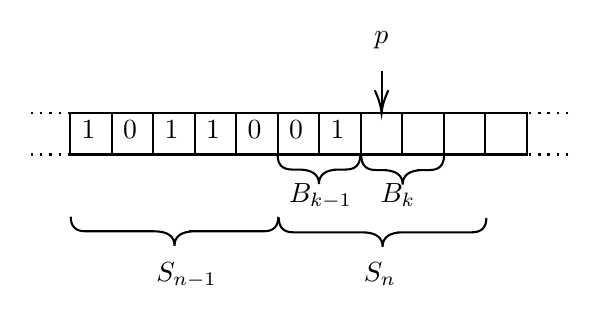
\begin{tikzpicture}[x=0.75pt,y=0.75pt,yscale=-1,xscale=1]
		%uncomment if require: \path (0,300); %set diagram left start at 0, and has height of 300

		%Shape: Rectangle [id:dp07152433688787241] 
		\draw   (100,100) -- (320,100) -- (320,120) -- (100,120) -- cycle ;
		%Straight Lines [id:da2936448051112307] 
		\draw    (120,100) -- (120,120) ;
		%Straight Lines [id:da027036583121563318] 
		\draw    (140,100) -- (140,120) ;
		%Straight Lines [id:da7810766858201694] 
		\draw    (160,100) -- (160,120) ;
		%Straight Lines [id:da5001340947135379] 
		\draw    (180,100) -- (180,120) ;
		%Straight Lines [id:da3843632481846373] 
		\draw    (200,100) -- (200,120) ;
		%Straight Lines [id:da03824030730667982] 
		\draw    (220,100) -- (220,120) ;
		%Straight Lines [id:da15646574434271243] 
		\draw    (240,100) -- (240,120) ;
		%Straight Lines [id:da846809534956415] 
		\draw    (260,100) -- (260,120) ;
		%Straight Lines [id:da4897590587430042] 
		\draw    (280,100) -- (280,120) ;
		%Straight Lines [id:da4069787777904943] 
		\draw    (300,100) -- (300,120) ;
		%Straight Lines [id:da05219000701716625] 
		\draw    (250,80) -- (250,98) ;
		\draw [shift={(250,100)}, rotate = 270] [color={rgb, 255:red, 0; green, 0; blue, 0 }  ][line width=0.75]    (10.93,-3.29) .. controls (6.95,-1.4) and (3.31,-0.3) .. (0,0) .. controls (3.31,0.3) and (6.95,1.4) .. (10.93,3.29)   ;
		%Shape: Brace [id:dp37474184805141453] 
		\draw   (100.25,150) .. controls (100.25,154.67) and (102.58,157) .. (107.25,157) -- (140.25,157) .. controls (146.92,157) and (150.25,159.33) .. (150.25,164) .. controls (150.25,159.33) and (153.58,157) .. (160.25,157)(157.25,157) -- (193.25,157) .. controls (197.92,157) and (200.25,154.67) .. (200.25,150) ;
		%Shape: Brace [id:dp9417201733674553] 
		\draw   (200.5,150.5) .. controls (200.5,155.17) and (202.83,157.5) .. (207.5,157.5) -- (240.5,157.5) .. controls (247.17,157.5) and (250.5,159.83) .. (250.5,164.5) .. controls (250.5,159.83) and (253.83,157.5) .. (260.5,157.5)(257.5,157.5) -- (293.5,157.5) .. controls (298.17,157.5) and (300.5,155.17) .. (300.5,150.5) ;
		%Straight Lines [id:da1555835238266523] 
		\draw  [dash pattern={on 0.84pt off 2.51pt}]  (100,100) -- (80,100) ;
		%Straight Lines [id:da0928939361477803] 
		\draw  [dash pattern={on 0.84pt off 2.51pt}]  (100,120) -- (80,120) ;
		%Straight Lines [id:da19581834915337515] 
		\draw  [dash pattern={on 0.84pt off 2.51pt}]  (340,120) -- (320,120) ;
		%Straight Lines [id:da4107689408293117] 
		\draw  [dash pattern={on 0.84pt off 2.51pt}]  (340,100) -- (320,100) ;
		%Shape: Brace [id:dp9863486277907854] 
		\draw   (240.25,120.5) .. controls (240.25,125.17) and (242.58,127.5) .. (247.25,127.5) -- (250.17,127.5) .. controls (256.84,127.5) and (260.17,129.83) .. (260.17,134.5) .. controls (260.17,129.83) and (263.5,127.5) .. (270.17,127.5)(267.17,127.5) -- (273.08,127.5) .. controls (277.75,127.5) and (280.08,125.17) .. (280.08,120.5) ;
		%Shape: Brace [id:dp8556326349440747] 
		\draw   (199.92,120.25) .. controls (199.92,124.92) and (202.25,127.25) .. (206.92,127.25) -- (209.83,127.25) .. controls (216.5,127.25) and (219.83,129.58) .. (219.83,134.25) .. controls (219.83,129.58) and (223.16,127.25) .. (229.83,127.25)(226.83,127.25) -- (232.75,127.25) .. controls (237.42,127.25) and (239.75,124.92) .. (239.75,120.25) ;

		% Text Node
		\draw (245,59.4) node [anchor=north west][inner sep=0.75pt]    {$p$};
		% Text Node
		\draw (104,102.4) node [anchor=north west][inner sep=0.75pt]    {$1$};
		% Text Node
		\draw (124,102.4) node [anchor=north west][inner sep=0.75pt]    {$0$};
		% Text Node
		\draw (144,102.4) node [anchor=north west][inner sep=0.75pt]    {$1$};
		% Text Node
		\draw (224,102.4) node [anchor=north west][inner sep=0.75pt]    {$1$};
		% Text Node
		\draw (164,102.4) node [anchor=north west][inner sep=0.75pt]    {$1$};
		% Text Node
		\draw (204,102.4) node [anchor=north west][inner sep=0.75pt]    {$0$};
		% Text Node
		\draw (240,170.4) node [anchor=north west][inner sep=0.75pt]    {$S_{n}$};
		% Text Node
		\draw (140,170.4) node [anchor=north west][inner sep=0.75pt]    {$S_{n-1}$};
		% Text Node
		\draw (248,132.4) node [anchor=north west][inner sep=0.75pt]    {$B_{k}$};
		% Text Node
		\draw (204,132.4) node [anchor=north west][inner sep=0.75pt]    {$B_{k-1}$};
		% Text Node
		\draw (184,102.4) node [anchor=north west][inner sep=0.75pt]    {$0$};
	\end{tikzpicture}
	\caption{Calcolo di $\mathbf{rank_b}(p)$.}
	\label{fig:example_rank_p}
\end{figure}

Quanto tempo impiega un'implementazione basata su queste strutture per
calcolare il rango di una posizione $p$? Per sapere quanti $1$ ci sono
prima della posizione $p$, bisogna innanzitutto calcolare il superblocco
di appartenenza di $p$, che è il superblocco numero $\frac{p}{\log_2(n)^2}$.
Vogliamo sapere quanti $1$ ci sono prima di quel superblocco - valore che abbiamo
memorizzato nei $S_i$. A questo punto, è necessario calcolare il numero di $1$
dall'inizio del superblocco all'inizio del blocco al quale appartiene $p$, valore salvato
in $B_i$. Rimane, quindi, da capire quanti $1$ ci sono dall'inizio del blocco al
quale appartiene $p$ fino alla posizione $p$ stessa. Per questo si può
utilizzare la tabella $Tab$ del four-russians trick:

$$
	\mathbf{rank}_{\mathbf{b}}(p) = S_{\frac{p}{\log_2(n)^2}} + B_{\frac{p}{\frac{1}{2}\log_2(n)}}
	+ Tab[t, p \mod \frac{1}{2}\log_2(n)]
$$
dove $t$ è il tipo blocco a cui $p$ appartiene secondo l'enumerazione dei blocchi di
$Tab$, calcolabile data la posizione d'inizio del blocco di $p$
$$
	x = \lfloor \frac{p}{\frac{1}{2}\log_2(n)}\rfloor (\frac{1}{2}\log_2(n))
$$
accedendo il vettore $\mathbf{b}$ e leggendo i valori del blocco\footnote{
	In termini pratici, come avviene questo accesso? Se avviene leggendo,
	uno per uno, tutti i valori del blocco al quale appartiene $p$ per poi
	accedere alla tabella $Tab$, non ha più senso leggere i valori da
	$\mathbf{b}[x]$ fino a $\mathbf{b}[p-1]$ contando gli $1$ visti?
}:
$$
	t = \mathbf{b}[x, x +1, \cdots, x + \frac{1}{2} \log_2(n) -1 ]
$$
Il calcolo del rank avviene quindi in tempo lineare,
poiché si tratta di accedere a $3$ tabelle e la struttura quindi
occupa lo spazio di $n + o(n)$ bit, poiché è necessario mantenere $b$ e
risponde alle query in tempo $O(1)$. Rispetto alla nostra classificazione,
questa struttura è \textbf{succinta} e ha la stessa efficienza della struttura naïve.

\subsection{Struttura di Clarke per la selezione}
La struttura di Clarke per la selezione è succinta teoricamente, ma in pratica
è raramente utilizzata perché la sua implementazione è molto complessa.
L'obiettivo è, dato un vettore $\mathbf{b}$ di valori binari fissato, calcolare
la funzione di selezione
$$
	\mathbf{select_b}(k) = \text{ posizione del } k-\text{esimo } 1
$$
La struttura di Clarke utilizza dei \textit{livelli}, simili a quelli utilizzati
dalla struttura di Jacobson.

\subsubsection{Primo livello}
Il primo livello della struttura di Clarke si è un insieme
di valori che rappresentano le posizioni degli $1$ di ordinalità multipla di
$\log_2(n) \cdot \log_2(\log_2(n))$, ossia
$$
	P_i =  \mathbf{select_b}(i \cdot \log_2(n) \cdot \log_2(\log_2(n)))
$$
ossia la posizione del $(i \cdot \log_2(n) \cdot \log_2(\log_2(n)))$-esimo $1$.

\paragraph{Memoria}
La grandezza di questa famiglia, ossia il numero di $P_i$, dipende dal
numero di $i$ che ci sono in $\mathbf{b}$, ma nel caso peggiore, il vettore
è composto unicamente da $1$ e vi saranno $\frac{n}{\log_2(n) \cdot \log_2(\log_2(n))}$ membri.
Ad ognuno di essi va associato un elemento, il quale richiede $\log_2(n)$ bit;
in totale, questo livello occupa
$$
	\frac{n}{\log_2(n) \cdot \log_2(\log_2(n))} \cdot \log_2(n) = o(n) \text{ bit}
$$

\subsubsection{Secondo livello}
Per le posizioni che non sono multiple di $\log_2(n) \cdot \log_2(\log_2(n))$ si utilizza
un secondo livello, che è costruito differentemente in base ad un indice calcolato
per ogni $P_i$:

$$
	\forall i ~ r_i = P_{i + 1} - P_i
$$
che rappresenta la distanza fra l'$(i \cdot \log_2(n) \cdot \log_2(\log_2(n)))$-esimo $1$
e il $((i+1) \cdot \log_2(n) \cdot \log_2(\log_2(n)))$-esimo. Questo
valore, $r_i$, sarà esattamente uguale a $\log_2(n) \cdot \log_2(\log_2(n))$ se e solo se
tra $P_{i}$ e $P_{i+1}$ ci sono unicamente $1$, e sarà maggiore se invece le
due posizioni sono più lontane.
% @TODO: serve un esempio, non si capisce bene. 
I due casi che si considerano dipendono dal valore di $r_i$.

\paragraph{Caso sparso}
Se $r_i \geq (\log_2(n) \cdot \log_2(\log_2(n)))^2$, significa che in $\mathbf{b}$ ci
sono pochi $1$ tra le posizioni $P_{i}$ e $P_{i+1}$; in questo caso
definiamo $S_i$ come la lista esplicita delle posizioni di tutti gli $1$
in $\mathbf{b}$ tra le due posizioni rappresentate come differenza tra $P_i$.

In questo caso, gli $S_i$ costruiti sono esattamente $\log_2(n)\cdot \log_2(\log_2(n))$,
in quanto stiamo contando gli $1$ in $\mathbf{b}$ tra il $(i \cdot \log_2(n) \cdot \log_2(\log_2(n))$-esimo
$1$ e il $((i+1) \cdot \log_2(n) \cdot \log_2(\log_2(n))$-esimo $1$, e ad ognuno
di essi si associa un numero che in grandezza è minore o uguale a
$\log_2(r_i)$, concludendo che per memorizzare un $S_i$ sono necessari
\begin{align*}
	\log_2(n)\cdot \log_2(\log_2(n)) \cdot \log_2(r_i) & = \frac{(\log_2(n)\cdot \log_2(\log_2(n)))^2}{\log_2(n)\cdot \log_2(\log_2(n))} \cdot \log_2(r_i) \\
	                                                   & \leq \frac{r_i}{\log_2(n)\cdot \log_2(\log_2(n))} \cdot \log_2(r_i)                               \\
	                                                   & \leq \frac{r_i}{\log_2(n)\cdot \log_2(\log_2(n))} \cdot \log_2(n)                                 \\
	                                                   & \leq \frac{r_i}{\log_2(\log_2(n))}                                                                \\
	                                                   & \leq \frac{n}{\log_2(\log_2(n))}   = o(n) \text{ bit}
\end{align*}

\paragraph{Caso denso}
Se $r_i \le (\log_2(n) \cdot \log_2(\log_2(n)))^2$, si memorizzano gli $1$
multipli di $\log_2(r_i)\log_2(\log_2(n))$, ossia partendo dalla posizione $P_i$ si salvano le
posizioni degli $j \cdot \log_2(r_i)\log_2(\log_2(n))$-esimi $1$ come differenze da $P_i$, ossia
$$
	S^i_j = \mathbf{select_b}(j \cdot \log_2(r_i)\log_2(\log_2(n))) - P_i
$$

In questo caso, gli $1$ memorizzati sono $\frac{\log_2(n)\cdot \log_2(\log_2(n))}{\log_2(r_i)\cdot \log_2(\log_2(n))}$.
Ad ognuno di questi si associa un valore in grandezza $\log_2(r_i)$, quindi lo spazio utilizzato
per memorizzare tutti i valori $S^i_j$ sono
$$
	\frac{\log_2(n)\cdot \log_2(\log_2(n))}{\log_2(r_i)\cdot \log_2(\log_2(n))} \log_2(r_i) =
	\frac{\log_2(n)\cdot \log_2(\log_2(n))}{\log_2(\log_2(n))} \leq \frac{r_i}{\log_2(\log_2(n))}
	\leq \frac{n}{\log_2(\log_2(n))} = o(n) \text{ bit}
$$


\subsubsection{Terzo livello}
Se nel secondo livello ci si trova nel caso denso, si utilizza un terzo livello.
Questo livello viene utilizzato esclusivamente per gli $1$ le cui posizioni non sono state
salvate nel secondo livello nel caso denso; pertanto, l'assunto è che
$$
	r_i < (\log_2(n) \log_2(\log_2(n)))^2
$$
Per ognuna di queste posizioni calcoliamo la differenza tra $S^i_j$:
$$
	\forall j \bar{r}^i_j = S^i_{j+1} - S^i_j
$$
Come nel caso precedente, abbiamo due possibilità in base al valore di $\bar{r}^i_j$, il quale
gode comunque della proprietà
$$
	\forall i, j ~~  \bar{r}^i_j \geq \log_2(r_i) \log_2(\log_2(n))
$$
\paragraph{Caso sparso}
Nel caso in cui $\bar{r}^i_j \geq \log_2(\bar{r}^i_j) \log_2(r_i) \log_2(\log_2(n))^2$,
si memorizzano esplicitamente tutte le posizioni degli $1$ tra $S^i_j$ e $S^i_{j+1}$
con dei valori $T^i_{j,k}$ come differenze tra $S^i_j$. In questo caso,
il consumo di memoria è
$$
	(\log_2(r_i)\cdot \log_2(\log_2(n)) \cdot \log_2(\bar{r}^i_j) \leq
	\frac{\log_2(r_i) \cdot \log_2(\log_2(n))^2 \log_2(\bar{r}^i_j)}{\log_2(\log_2(n))}
	\leq \frac{\bar{r}^i_j}{\log_2(\log_2(n))} = o(n) \text{ bit}
$$
\paragraph{Caso denso}
Nel caso in cui $\bar{r}^i_j \le \log_2(\bar{r}^i_j) \log_2(r_i) \log_2(\log_2(n))^2$,
significa che ci sono pochi $0$ tra $S^i_j$ e $S^i_{j+1}$ e
si utilizza il four-russians trick. Inizialmente osserviamo quanto segue.
\begin{oss}
	\begin{align*}
		\log_2(\bar{r}^i_j) \leq \log_2(r_i) & \leq \log_2(\log_2(n)\cdot \log_2(\log_2(n)))^2     \\
		                                     & = 2 \log_2(\log_2(n)) + 2 \log_2(\log_2(\log_2(n))) \\
		                                     & \leq 4 \log_2(\log_2(n))
	\end{align*}
\end{oss}
\begin{oss}
	$$
		\bar{r}^i_j < \log_2(\bar{r}^i_j) \cdot \log_2(r_i) \cdot (\log_2(\log_2(n))^2
		\leq 16(\log_2\log_2(n))^4
	$$
\end{oss}
Lo spazio necessario per utilizzare il four-russians trick è quanto segue.
Servono $2^{\bar{r}^i_j}$ enumerazioni di `sottovettori',
ossia la dimensione tra $S^i_j$ e $S^i_{j+1}$,
che è la parte che va memorizzata esplicitamente; per ognuna di queste
enumerazioni è necessario salvare la posizione di $\bar{r}^i_j$ $1$ utilizzando
memoria al massimo $\log_2(\bar{r}^i_j)$:
\begin{align*}
	2^{\bar{r}^i_j} \cdot \bar{r}^i_j \cdot \log_2(\bar{r}^i_j) & \leq
	2^{16(\log_2\log_2(n))^4} \cdot 16(\log_2\log_2(n))^4 \cdot \log_2(16(\log_2\log_2(n))^4)                                  \\
	                                                            & = 16(\log_2\log_2(n))^8 \log_2(16(\log_2\log_2(n))^4) = o(n)
\end{align*}


\subsubsection{Complessità totale in spazio}
In totale, per memorizzare $\mathbf{b}$ e i possibili tre livelli di struttura,
sono necessari $o(n)$ bit per il primo livello e, in base a come è fatto il secondo livello
$$
	\sum^{\frac{n}{\log_2(n)\cdot \log_2(\log_2(n))}} \frac{P_{i+1} - P_i}{\log_2(\log_2(n)}
	= \frac{P_n - P_0}{\log_2(\log_2(n))}
	\leq \frac{n}{\log_2(\log_2(n))} = o(n) \text{ bit}
$$
più $o(n)$ bit per il terzo livello. Quindi, la struttura di Clarke occupa
spazio $n + o(n)$ e ha accesso tempo di accesso costante, pertanto è
una struttura \textbf{succinta}.

\begin{figure}
	\centering
	\tikzset{every picture/.style={line width=0.75pt}} %set default line width to 0.75pt        

	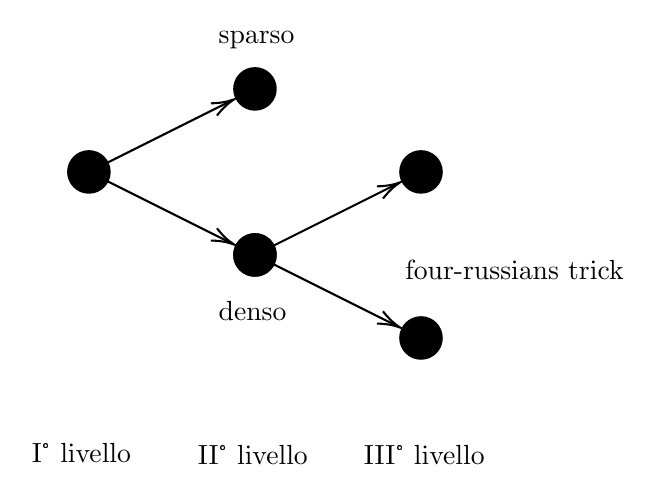
\begin{tikzpicture}[x=0.75pt,y=0.75pt,yscale=-1,xscale=1]
		%uncomment if require: \path (0,300); %set diagram left start at 0, and has height of 300

		%Shape: Circle [id:dp9914836432536758] 
		\draw  [fill={rgb, 255:red, 0; green, 0; blue, 0 }  ,fill opacity=1 ] (70,101) .. controls (70,95.48) and (74.48,91) .. (80,91) .. controls (85.52,91) and (90,95.48) .. (90,101) .. controls (90,106.52) and (85.52,111) .. (80,111) .. controls (74.48,111) and (70,106.52) .. (70,101) -- cycle ;
		%Shape: Circle [id:dp09703813871749656] 
		\draw  [fill={rgb, 255:red, 0; green, 0; blue, 0 }  ,fill opacity=1 ] (150,61) .. controls (150,55.48) and (154.48,51) .. (160,51) .. controls (165.52,51) and (170,55.48) .. (170,61) .. controls (170,66.52) and (165.52,71) .. (160,71) .. controls (154.48,71) and (150,66.52) .. (150,61) -- cycle ;
		%Straight Lines [id:da8346853138498954] 
		\draw    (80,101) -- (148.21,66.89) ;
		\draw [shift={(150,66)}, rotate = 153.43] [color={rgb, 255:red, 0; green, 0; blue, 0 }  ][line width=0.75]    (10.93,-3.29) .. controls (6.95,-1.4) and (3.31,-0.3) .. (0,0) .. controls (3.31,0.3) and (6.95,1.4) .. (10.93,3.29)   ;
		%Shape: Circle [id:dp4565729376211175] 
		\draw  [fill={rgb, 255:red, 0; green, 0; blue, 0 }  ,fill opacity=1 ] (150,141) .. controls (150,146.52) and (154.48,151) .. (160,151) .. controls (165.52,151) and (170,146.52) .. (170,141) .. controls (170,135.48) and (165.52,131) .. (160,131) .. controls (154.48,131) and (150,135.48) .. (150,141) -- cycle ;
		%Straight Lines [id:da8127484960209145] 
		\draw    (80,101) -- (148.21,135.11) ;
		\draw [shift={(150,136)}, rotate = 206.57] [color={rgb, 255:red, 0; green, 0; blue, 0 }  ][line width=0.75]    (10.93,-3.29) .. controls (6.95,-1.4) and (3.31,-0.3) .. (0,0) .. controls (3.31,0.3) and (6.95,1.4) .. (10.93,3.29)   ;
		%Shape: Circle [id:dp546530222511162] 
		\draw  [fill={rgb, 255:red, 0; green, 0; blue, 0 }  ,fill opacity=1 ] (150,141) .. controls (150,135.48) and (154.48,131) .. (160,131) .. controls (165.52,131) and (170,135.48) .. (170,141) .. controls (170,146.52) and (165.52,151) .. (160,151) .. controls (154.48,151) and (150,146.52) .. (150,141) -- cycle ;
		%Shape: Circle [id:dp1691093585413369] 
		\draw  [fill={rgb, 255:red, 0; green, 0; blue, 0 }  ,fill opacity=1 ] (230,101) .. controls (230,95.48) and (234.48,91) .. (240,91) .. controls (245.52,91) and (250,95.48) .. (250,101) .. controls (250,106.52) and (245.52,111) .. (240,111) .. controls (234.48,111) and (230,106.52) .. (230,101) -- cycle ;
		%Straight Lines [id:da17118221437478087] 
		\draw    (160,141) -- (228.21,106.89) ;
		\draw [shift={(230,106)}, rotate = 153.43] [color={rgb, 255:red, 0; green, 0; blue, 0 }  ][line width=0.75]    (10.93,-3.29) .. controls (6.95,-1.4) and (3.31,-0.3) .. (0,0) .. controls (3.31,0.3) and (6.95,1.4) .. (10.93,3.29)   ;
		%Shape: Circle [id:dp8870903616648642] 
		\draw  [fill={rgb, 255:red, 0; green, 0; blue, 0 }  ,fill opacity=1 ] (230,181) .. controls (230,186.52) and (234.48,191) .. (240,191) .. controls (245.52,191) and (250,186.52) .. (250,181) .. controls (250,175.48) and (245.52,171) .. (240,171) .. controls (234.48,171) and (230,175.48) .. (230,181) -- cycle ;
		%Straight Lines [id:da2110125336208042] 
		\draw    (160,141) -- (228.21,175.11) ;
		\draw [shift={(230,176)}, rotate = 206.57] [color={rgb, 255:red, 0; green, 0; blue, 0 }  ][line width=0.75]    (10.93,-3.29) .. controls (6.95,-1.4) and (3.31,-0.3) .. (0,0) .. controls (3.31,0.3) and (6.95,1.4) .. (10.93,3.29)   ;

		% Text Node
		\draw (51,230) node [anchor=north west][inner sep=0.75pt]   [align=left] {I° livello};
		% Text Node
		\draw (131,231) node [anchor=north west][inner sep=0.75pt]   [align=left] {II° livello};
		% Text Node
		\draw (211,231) node [anchor=north west][inner sep=0.75pt]   [align=left] {III° livello};
		% Text Node
		\draw (141,162) node [anchor=north west][inner sep=0.75pt]   [align=left] {denso};
		% Text Node
		\draw (141,32) node [anchor=north west][inner sep=0.75pt]   [align=left] {sparso};
		% Text Node
		\draw (231,142) node [anchor=north west][inner sep=0.75pt]   [align=left] {four-russians trick};
	\end{tikzpicture}
	\caption{Struttura di Clarke per la selezione.}
\end{figure}



% lezione 19 - 01-12-2021
\section{Strutture succinte per alberi binari}
Gli \textit{alberi} possono essere visti in due modi: per i
matematici, essi sono dei grafi connessi aciclici mentre per gli
informatici sono una \textit{struttura dati} radicata che ha una
\textit{radice}. In particolare, un albero \textit{binario} è un
albero tale per cui ogni nodo ha al più due figli; formalmente,
si definiscono induttivamente: l'albero con un solo nodo (che è anche
la radice), denotato $\emptyset$, è un albero binario;
se $T_1$ e $T_2$ sono due alberi binari,
allora anche l'albero radicato in un nuovo nodo che ha come figli
$T_1$ e $T_2$, denotato $(T_1, T_2)$ è un albero binario. In questa definizione,
ogni nodo ha o $0$ o $2$ figli. I nodi che non hanno figli
sono chiamati \textbf{nodi esterni} o \textbf{foglie}, mentre gli altri sono
chiamati \textbf{nodi interni}.


\begin{figure}[!hb]
	\begin{subfigure}{0.45\textwidth}
		\begin{center}
			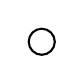
\begin{tikzpicture}
				\node [circle, draw]{};
			\end{tikzpicture}
		\end{center}
		\caption{L'albero binario $\emptyset$.}
	\end{subfigure}
	\begin{subfigure}{0.45\textwidth}
		\begin{center}
			\begin{tikzpicture}
				\node [circle,draw]{}
				child {node [isosceles triangle,draw,shape border rotate=90] {$T_1$}}
				child {node [isosceles triangle,draw,shape border rotate=90] {$T_2$}};
			\end{tikzpicture}
		\end{center}
		\caption{L'albero binario $(T_1, T_2)$.}
	\end{subfigure}
	\caption{Definizione induttiva di albero binario.}
	\label{fig:btree_inductive}
\end{figure}

\begin{figure}
	\begin{center}
		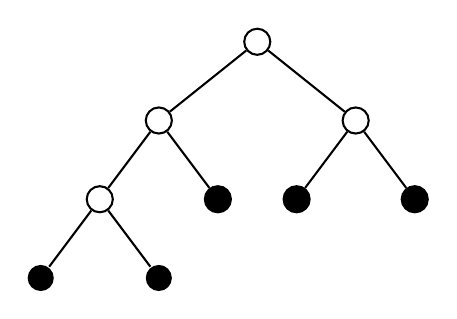
\begin{tikzpicture}
			\node [circle,draw]{} [level distance=10mm,sibling distance=25mm]
			child { node [circle,draw]{} [level distance=10mm ,sibling distance=15mm]
					child {node [circle,draw] {}
							child {node [circle,fill] {}}
							child {node [circle,fill]{}}}
					child {node [circle,draw,fill]{}}
				}
			child {node [circle,draw] {} [level distance=10mm ,sibling distance=15mm]
					child {node [circle,draw,fill] {}}
					child {node [circle,draw,fill]{}}
				};
		\end{tikzpicture}
	\end{center}
	\caption{L'albero binario $(((\emptyset, \emptyset), \emptyset), (\emptyset, \emptyset))$.}
	\label{fig:btree_example}
\end{figure}

\noindent
Ora stiamo descrivendo alberi \textit{vuoti}, ossia che non contengono dati:
alternative sono gli alberi \textbf{ancillari}, i quali contengono dati solo nei nodi interni
o solo nelle foglie. Al netto di queste distinzioni, definiamo $E$ l'insieme dei nodi
esterni, $I$ l'insieme dei nodi interni di un albero binario e $n$ il numero di nodi
interni, ossia $n = |I|$. Inoltre, `equipaggiamo' gli alberi binari di due funzioni
$ext$ e $int$, che denotano l'insieme delle foglie interne e l'insieme delle foglie
interne di un albero binario.

\begin{theorem} \label{thm:btree_leaves}
	In ogni albero binario, il numero di foglie in un albero binario è uguale al numero di nodi esterni più uno:
	$$
		|E| = |I| + 1
	$$
\end{theorem}
\begin{proof}
	Per induzione.
	\begin{itemize}
		\item{\bf base}: $ext(\emptyset) = 1$ e $int(\emptyset) = 0$.
		\item{\bf induzione}: siano $L, R$ due alberi binari. Allora
		$$
			ext((L,R)) = ext(L) + ext(R) = int(L) + 1 + int(R) + 1 = int((L, R))  + 1
		$$
	\end{itemize}
\end{proof}

\begin{corollario}
	Ogni albero con $n$ nodi interni ha in totale $2n +1$ nodi.
\end{corollario}

\begin{theorem}[di Catalan]\label{thm:catalan}
	Il numero di alberi binari con $n$ nodi interni è
	$$
		C_n = \frac{1}{n+1}{2n \choose n}
	$$
\end{theorem}
\begin{proof}
	Omessa.
\end{proof}
\begin{corollario}
	$ \forall n ~ \log_2(C_n)  =2n + O(\log_2(n)) $
\end{corollario}
\begin{proof}
	Utilizzando l'approssimazione di Sterling
	$$
		x! \approx \sqrt{2\pi x} (\frac{x}{e})^x
	$$

	si ha che
	$$
		C_n = \frac{1}{n+1} \frac{(2n)!}{n! (2n - n)!} = \frac{1}{n+1}\frac{(2n)!}{(n!)^2} \approx
		\frac{1}{n+1} \frac{\sqrt{4 \pi n} (\frac{2n}{e})^{2n}}{2 \pi n (\frac{n}{e})^{2n}}
		= \frac{1}{n+1} \frac{1}{\sqrt{\pi n }} 2^{2n} \approx \frac{4^n}{\sqrt{\pi n^3}}
	$$
	(che può essere dimostrato asintoticamente corretto).
	Questo significa che
	$$
		\log_2(C_n) = n \log_2(4) - \frac{1}{2}\log_2(\pi n^3)
		= 2n - \frac{3}{2}\log_2(n) - \frac{1}{2}\log_2(\pi)
		= 2n + O(\log_2(n))
	$$
\end{proof}
\begin{corollario}
	Per memorizzare alberi binari con $n$ nodi interni sono necessari
	$$
		Z_n = 2n + O(\log_2(n)) \text{ bit}
	$$
\end{corollario}

\subsection{Rappresentazione}

Per rappresentare un albero binario con $n$ nodi interni, numeriamo seguendo una visita in
ampiezza i nodi dell'albero, come rappresentato in \cref{fig:btree_rappr_num}. I numeri assegnati
andranno da $0$ a $2n$.

\begin{figure}[h]
	\centering
	\begin{subfigure}[t]{0.45\textwidth}
		\centering
		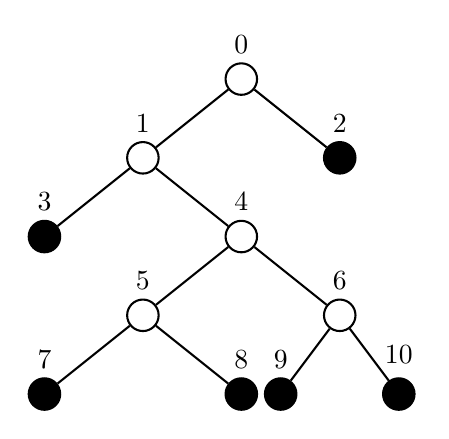
\begin{tikzpicture}[
				every node/.style={circle, draw, minimum size=4mm, inner sep=0.5mm},
				level distance=10mm,
				level 1/.style={sibling distance=25mm},
				level 2/.style={sibling distance=25mm}]
			\node [label=above:{0}]{}
			child {
			node [label=above:{1}] {}
			child {node[fill, label=above:{3}]{}}
			child {
			node[label=above:{4}]{}
			child {
			node [label=above:{5}]{}
			child {node[fill,label=above:{7}]{}}
			child {node[fill,label=above:{8}]{}}
			}
			child {
			node[label=above:{6}]  {}
			[level distance=10mm ,sibling distance=15mm]
			child {node[fill,label=above:{9}] {}}
			child {node[fill,label=above:{10}] {}}
			}
			}
			}
			child {node [fill, label=above:{2}]{}};
		\end{tikzpicture}

		\caption{L'albero binario $((\emptyset, ((\emptyset, \emptyset), (\emptyset, \emptyset))), \emptyset)$ numerato.}
		\label{fig:btree_rappr_num}

	\end{subfigure}
	\begin{subfigure}[t]{0.45\textwidth}
		\centering
		\tikzset{every picture/.style={line width=0.75pt}} %set default line width to 0.75pt        

		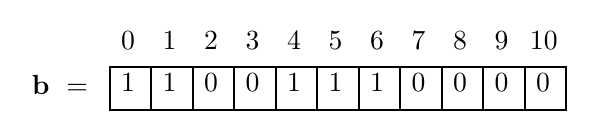
\begin{tikzpicture}[x=0.75pt,y=0.75pt,yscale=-1,xscale=1]
			%uncomment if require: \path (0,300); %set diagram left start at 0, and has height of 300

			%Shape: Rectangle [id:dp4589196649246813] 
			\draw   (160,120) -- (180,120) -- (180,140.67) -- (160,140.67) -- cycle ;
			%Shape: Rectangle [id:dp7482491218517459] 
			\draw   (180,120) -- (200,120) -- (200,140.67) -- (180,140.67) -- cycle ;
			%Shape: Rectangle [id:dp3055160865785119] 
			\draw   (200,120) -- (220,120) -- (220,140.67) -- (200,140.67) -- cycle ;
			%Shape: Rectangle [id:dp6460750266770654] 
			\draw   (220,120) -- (240,120) -- (240,140.67) -- (220,140.67) -- cycle ;
			%Shape: Rectangle [id:dp45180487257490853] 
			\draw   (240,120) -- (260,120) -- (260,140.67) -- (240,140.67) -- cycle ;
			%Shape: Rectangle [id:dp28629681352535363] 
			\draw   (260,120) -- (280,120) -- (280,140.67) -- (260,140.67) -- cycle ;
			%Shape: Rectangle [id:dp7936708770675233] 
			\draw   (280,120) -- (300,120) -- (300,140.67) -- (280,140.67) -- cycle ;
			%Shape: Rectangle [id:dp23915136536136594] 
			\draw   (300,120) -- (320,120) -- (320,140.67) -- (300,140.67) -- cycle ;
			%Shape: Rectangle [id:dp722227591081337] 
			\draw   (320,120) -- (340,120) -- (340,140.67) -- (320,140.67) -- cycle ;
			%Shape: Rectangle [id:dp6052306075858915] 
			\draw   (340,120) -- (360,120) -- (360,140.67) -- (340,140.67) -- cycle ;
			%Shape: Rectangle [id:dp5583026074292488] 
			\draw   (360,120) -- (380,120) -- (380,140.67) -- (360,140.67) -- cycle ;

			% Text Node
			\draw (121,122.4) node [anchor=north west][inner sep=0.75pt]    {$\mathbf{b} \ =\ $};
			% Text Node
			\draw (164,101.4) node [anchor=north west][inner sep=0.75pt]    {$0$};
			% Text Node
			\draw (184,101.4) node [anchor=north west][inner sep=0.75pt]    {$1$};
			% Text Node
			\draw (204,101.4) node [anchor=north west][inner sep=0.75pt]    {$2$};
			% Text Node
			\draw (224,101.4) node [anchor=north west][inner sep=0.75pt]    {$3$};
			% Text Node
			\draw (244,101.4) node [anchor=north west][inner sep=0.75pt]    {$4$};
			% Text Node
			\draw (264,101.4) node [anchor=north west][inner sep=0.75pt]    {$5$};
			% Text Node
			\draw (284,101.4) node [anchor=north west][inner sep=0.75pt]    {$6$};
			% Text Node
			\draw (304,101.4) node [anchor=north west][inner sep=0.75pt]    {$7$};
			% Text Node
			\draw (324,101.4) node [anchor=north west][inner sep=0.75pt]    {$8$};
			% Text Node
			\draw (344,101.46) node [anchor=north west][inner sep=0.75pt]    {$9$};
			% Text Node
			\draw (361,101.4) node [anchor=north west][inner sep=0.75pt]    {$10$};
			% Text Node
			\draw (164,121.4) node [anchor=north west][inner sep=0.75pt]    {$1$};
			% Text Node
			\draw (184,121.4) node [anchor=north west][inner sep=0.75pt]    {$1$};
			% Text Node
			\draw (204,121.4) node [anchor=north west][inner sep=0.75pt]    {$0$};
			% Text Node
			\draw (224,121.4) node [anchor=north west][inner sep=0.75pt]    {$0$};
			% Text Node
			\draw (244,121.4) node [anchor=north west][inner sep=0.75pt]    {$1$};
			% Text Node
			\draw (264,121.4) node [anchor=north west][inner sep=0.75pt]    {$1$};
			% Text Node
			\draw (284,121.4) node [anchor=north west][inner sep=0.75pt]    {$1$};
			% Text Node
			\draw (304,121.4) node [anchor=north west][inner sep=0.75pt]    {$0$};
			% Text Node
			\draw (324,121.4) node [anchor=north west][inner sep=0.75pt]    {$0$};
			% Text Node
			\draw (344,121.46) node [anchor=north west][inner sep=0.75pt]    {$0$};
			% Text Node
			\draw (364,121.4) node [anchor=north west][inner sep=0.75pt]    {$0$};

		\end{tikzpicture}
		\caption{Vettore $\mathbf{v}$ associato.}
		\label{fig:btree_rappr_vec}
	\end{subfigure}
	\caption{}
\end{figure}

La concreta rappresentazione dell'albero si realizza con un vettore di bit di lunghezza
$2n + 1$ $\mathbf{v}$ tale che
$$
	\forall i ~ \mathbf{v}[i] =
	\begin{cases}
		1 & i \in I \\
		0 & i \in E
	\end{cases}
$$
ottenendo quindi esattamente $n$ `$1$' nel vettore, come esemplificato in \cref{fig:btree_rappr_vec}.

Si immagini di avere l'albero binario in cui vi è un nodo interno numerato $p$
con due figli con numeri $q$ e $q+1$, come in \cref{fig:btree_rappr_step}.
Chiaramente si ha $Q = |nodi di T'| = 2 |nodi interni di T'| + 1 = 2(|nodi interni di T| < P) + 1 = 2(|uni dentro il vettore b di indice p +1 = 2rank_b(P) +1$.
Se invece è necessario anche risalire al genitore a partire dal figlio, allora il figlio di sinistra è
$2rank_b(q) +1 = P$, mentre il figlio di destra è $2rank_b(q) + 2 = P$, quindi
$$
	\begin{cases}
		rank_b(q) = \frac{P}{2} - \frac{1}{2} \\
		rank_b(q) = \frac{P}{2} - 1           \\
	\end{cases}
	= rank_b(q) = \lfloor\frac{P}{2} - {1}{2} \rfloor
$$
$select(rank_b(q)) = select(\lfloor\frac{P}{2} - {1}{2} \rfloor) \implies q = select(\lfloor\frac{P}{2} - {1}{2}\rfloor)$
indipendentemente dal fatto che $q$ sia figlio di destra o di sinistra.


Per rappresentare un albero con $n$ nodi interni utilizziamo un vettore $b$ che ha tanti
bit tanti quanti sono i nodi dell'albero, ossia $2n +1$. Oltre a questo, si utilizza
lo spazio utilizzato dalle strutture di rank e select, ossia
$$
	D_n = 2n +1 + o(2n+1) = 2n + 1 + o(n)
$$
con un risultato per $Z_n$ pari a $2n + O(\log_1(n))$, la differenza è
$$
	D_n - Z_n = o(n)
$$
pertanto la struttura è succinta con accesso in tempo costante.

\begin{figure}[h]
	\centering
	\tikzset{every picture/.style={line width=0.75pt}} %set default line width to 0.75pt        
	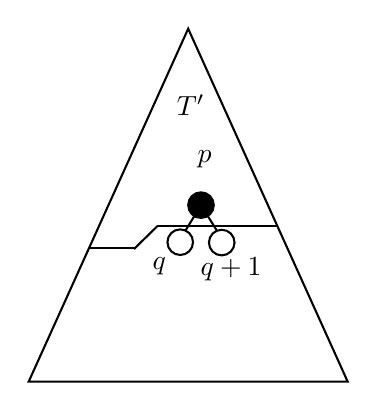
\begin{tikzpicture}[x=0.75pt,y=0.75pt,yscale=-1,xscale=1]
		%Shape: Circle [id:dp7169355320482411] 
		\draw  [fill={rgb, 255:red, 0; green, 0; blue, 0 }  ,fill opacity=1 ] (360.11,106.08) .. controls (360.11,102.68) and (362.87,99.92) .. (366.28,99.92) .. controls (369.68,99.92) and (372.44,102.68) .. (372.44,106.08) .. controls (372.44,109.49) and (369.68,112.25) .. (366.28,112.25) .. controls (362.87,112.25) and (360.11,109.49) .. (360.11,106.08) -- cycle ;
		%Straight Lines [id:da11031799115386731] 
		\draw    (366.28,106.08) -- (356.04,122.86) ;
		%Straight Lines [id:da5314879825236313] 
		\draw    (366.28,106.08) -- (376.09,121.82) ;
		%Shape: Triangle [id:dp2636274720755136] 
		\draw   (360.11,21.08) -- (436.94,191.08) -- (283.28,191.08) -- cycle ;
		%Straight Lines [id:da07107046785599602] 
		\draw    (312.18,126.95) -- (334.47,126.95) ;
		%Straight Lines [id:da23996966123276942] 
		\draw    (345.08,116.14) -- (402.93,116.14) ;
		%Straight Lines [id:da8657897153449609] 
		\draw    (345.49,115.99) -- (333.99,127.24) ;
		%Shape: Circle [id:dp6390655913899737] 
		\draw  [fill={rgb, 255:red, 255; green, 255; blue, 255 }  ,fill opacity=1 ] (350.11,123.93) .. controls (350.11,120.53) and (352.87,117.76) .. (356.28,117.76) .. controls (359.68,117.76) and (362.44,120.53) .. (362.44,123.93) .. controls (362.44,127.34) and (359.68,130.1) .. (356.28,130.1) .. controls (352.87,130.1) and (350.11,127.34) .. (350.11,123.93) -- cycle ;
		%Shape: Circle [id:dp31674144349432576] 
		\draw  [fill={rgb, 255:red, 255; green, 255; blue, 255 }  ,fill opacity=1 ] (370.11,124.11) .. controls (370.11,120.71) and (372.87,117.95) .. (376.28,117.95) .. controls (379.68,117.95) and (382.44,120.71) .. (382.44,124.11) .. controls (382.44,127.52) and (379.68,130.28) .. (376.28,130.28) .. controls (372.87,130.28) and (370.11,127.52) .. (370.11,124.11) -- cycle ;

		% Text Node
		\draw (341.53,130) node [anchor=north west][inner sep=0.75pt]    {$q$};
		% Text Node
		\draw (364.58,130) node [anchor=north west][inner sep=0.75pt]    {$q+1$};
		% Text Node
		\draw (363.18,78.26) node [anchor=north west][inner sep=0.75pt]    {$p$};
		% Text Node
		\draw (353.2,51.2) node [anchor=north west][inner sep=0.75pt]    {$T'$};


	\end{tikzpicture}
	\caption{}
	\label{fig:btree_rappr_step}
\end{figure}



\subsection{Alberi binari con dati}
Se i dati si trovano su ogni tipo di nodo dell'albero (sia interni che interni) i dati
\textit{ancillari} si possono mantenere in un ulteriore vettore della stessa lunghezza.
% disegno..
Se, invece, i dati ancillari si trovano esclusivamente sui nodi interni, la situazione è leggermente
più complicata: il vettore dei dati avrà lunghezza pare ai al numero di nodi interni: sarà quindi
necessario ottenere il numero del nodo interno, utilizzando quindi una \texttt{select}. Alternativamente,
se si vogliono salvare dati sulle foglie, si dovrà utilizzare una tecnica in grado di contare il \texttt{rank}
per gli $0$.

\section{Rappresentazione di Elias-Fano di sequenze monotone}
Una sequenza di interi
$$
	x_0, x_1, \cdots, x_{n+1}
$$
ordinati (ossia $i < j \implies x_i < x_j$) e tutti minori di un numero $u$ chiamato
\textit{dimensione dell'universo} (ossia $\forall i, x_i < u$) richiede una primitiva che, presentato
un indice $i$, restituisce l'$i$-esimo elemento della sequenza.

La rappresentazione di Elias-Fano
% 0  	0 	0 	0
% 0     0       0       0
% 1     1       1       1 			Parte superiore
% 1     1       1       1
% -------------------------- 			Limite l 
% 0     1       1       1 			
% 1     0       0       1 			Parte inferiore
% 0     0       1       0
$l = \max\{0, \lfloor \log_2{\frac{u}{n}}\rfloor\}$ assumiamo $u >= n$.

Le parti inferiori $l_i = x_i \mod 2^l$ vengono memorizzati esplicitamente, utilizzando $l$ bit per ciascuno.
Ciò che rimane è la parte superiore, ossia $s_i = \lfloor{\frac{x_{i}}{2^l}}\rfloor$ e chiamiamo
$$
	u_i = \lfloor{\frac{x_i}{2^l}}\rfloor -\lfloor{\frac{x_{i-1}}{2^l}}\rfloor
$$
assumendo $x_{-1} = 0$; questa sequenza di differenze viene memorizzata in unario, terminate dal bit $1$:
questa sequenza è salvata in un vettore $u$, sul quale viene costruita una struttura di rank e select.

Le due strutture, la lista di $l$ e il vettore $u$, utilizzano il seguente spazio:
$l$: $ln$ bit; $u$: $\sum_{i = 0}^{ n-1} (u_i + 1) = n + \sum_{i = 0}^{n-1} u_i = n + \sum_{i = 0}^{n-1} \lfloor{\frac{x_i}{2^l}}\rfloor -\lfloor{\frac{x_{i-1}}{2^l}}\rfloor$
che identifica una serie telescopica, nella quale rimarrà $u = n - \lfloor{\frac{x_{n-1}}{2^l}}\rfloor -\lfloor{\frac{x_{-1}}{2^l}}\rfloor \leq n + \frac{u}{2^l}$
$ = n + \frac{u}{2^{\lfloor log(\frac{u}{n})\rfloor}}$.
Se $u/n$ è una potenza di $2$, allora
$ = n + \frac{u}{(u/n)} = 2n$;
altrimenti
$ \leq n + \frac{u}{2^{log(\frac{u}{n}) - 1 }} = n + \frac{u}{2^{\log(u/n)}1/2} = n + \frac{2n}{u/n} = 3n$.
In tutto, quindi, si occupano
$(l+2)n$ bit o $(l+3)n$ bit, a seconda che $u/n$ sia potenza di $2$.
$$
	\lceil l = \log_2(u/n) \rceil =
	\begin{cases}
		l & u/n \text{ è una potenza di } 2 \\
		l +1                                \\
	\end{cases}
$$
concludiamo
$$
	D_n = (2 + \lceil \log_2(u/n) \rceil)
$$
che però non tiene conto dello spazio occupato da rank e select.

Supponiamo di volere la posizione dell'$i$-esimo $1$ in $u$:
$$
	select_u(i) = u_0 + u_1 \cdots + u_{i-1} + i
$$
Quindi $ select_u(i) - i = \sum_{j = 0}^i \lfloor{\frac{x_{j}}{2^l}}\rfloor -\lfloor{\frac{x_{j-1}}{2^l}}\rfloor  = \lfloor \frac{x_i}{2^l} \rfloor$;
di conseguenza $x_i =  \lfloor \frac{x_i}{2^l} \rfloor 2^l + x_i mod 2^l = (select_u(i) - i ) 2^l + l_i$.
E, contando anche le strutture di rank e select,
$$
	D_n = (2 + \lceil \log_2(u/n) \rceil)n + o(n)
$$

\subsubsection{Lower bound per le strutture di Elias-Fano}
Dobbiamo considerare tutte le sequenze monotone
$$
	0 \leq x_0 \leq \cdots \leq x_{n-1} \leq u
$$
Quante sono, una volta fissati $n$ e $u$? Esse sono in biiezioni con i multinsiemi di cardinalità
$n$ sottoinsiemi di $\{0,1, \cdots, u-1\}$. Uno di questi multinsiemi si può vedere come
$$
	c_0, c_1, \cdots, c_{u-1}
$$
che si può vedere come il numero di occorrenze del valore $0, 1, \cdots, u-1$ nel multinsieme, ossia
il numero di soluzioni intere non negative dell'equazione $c_0 + c_1, \cdots, c_{u-1} = n$. Quante sono le
soluzioni? Per farlo, si può utilizzare la tecnica \textit{stars and bands}.  Il numero di soluzioni
è uguale al numero di stringhe costruite in tale modo. In quanti modi si possono disporre le
$n$ stelline e le $u-1$ barrette? Si hanno in totale $u + n -1 $ caratteri; ossia ${u + n -1}\choose{u - 1}$.
Questo fornisce l'I.T.L.B:
$Z_n = \log_2({{u + n -1}\choose{u - 1}})$.
%
% Approx: (a choose b) \approx b log(a/b) + (a - b ) + log(a/(a-b))

$Z_n = \log_2({{u + n -1}\choose{u - 1}}) \approx = n \log_2(\frac{u + n -1) + (u + n -1 - u + 1) + log(\frac{u + n - 1}{\frac{u + n -1-u + 1}{u -1}}})$
$= n \log_2(\frac{u + n - 1}{n}) = n \log(u/n(1 + n/u - 1/u)) = n log(u/n) + log(1 + n/u - 1/u)$
% approx: x \approx ln(1+x)
$= Z_n \approx n log(u/n) + n ln(1 + n/u - 1/u) {1/\ln(2)} = n log (u/n) + n (n/u - 1/n) 1/ln2 = n log(u/n( + 1/n 1/log2) - n/u 1(ln2))$
$ Z_n \approx n \log_2(\frac{u}{n})$


numero di bit per elemento nel caso migliore:
$$
	\bar{Z}_n = log (u/n)
$$
$$
	\bar{D}_n = 2 + \lceil log(u/n) \rceil + o(n)
$$
$$
	\bar{Z}_n - \bar{D}_n = 2 + o(n) \implies \bar{D}_n = \bar{Z}_n + O(1)
$$
rendendo la struttura \textit{quasi}-implicita nel caso sparso; si può vedere che l'analisi funziona a patto che
$n \leq \sqrt(u)$.

\section{Strutture per parentesi ben formate}

DI ogni parentesi lontana possiamo guardare dove si chiude: due parentesi lontane in un blocco
si possono chiudere entrambe in un blocco più avanti; la prima viene chiamata \textit{pioniera}.
Essa è una parentesi lontana e
\begin{itemize}
	\item è la prima del blocco oppure
	\item è la prima a chiudersi in un certo blocco
\end{itemize}
Per rappresentare la parola memorizziamo, oltre a $w$, un vettore $p$ di $n$ bit con $1$ nelle posizioni
delle pioniere. Inoltre, teniamo altri tre vettori: $E$, che per ogni blocco $i$ da l'eccesso all'inizio
del blocco $i$ (quindi ha un elemento per ogni blocco); $M$, che per ogni blocco $i$ mantiene la posizione
della parentesi corrispondente all'$i$-esima pioniera e, infine, $O$ per ogni blocco $i$ mantiene la
posizione della prima aperta a sinistra dell'inizio di $i$ avente eccesso $x-1$, dove $x$ è il
minimo eccesso del blocco.

Lo spazio occupato da queste strutture è:
$$
	\begin{aligned}
		 & w &  & n                                                                  \\
		 & p &  & n + o(n)                                                           \\
		 & E &  & k + \log_2(n)                                                      \\
		 & O &  & k + \log_2(n)                                                      \\
		 & M &  & \text{pioniere} \cdot \log_2(n) < (4k - 6) \log_2(n) < 4k\log_2(n)
	\end{aligned}
$$
\begin{theorem}
	Se ci sono $k$ blocchi, vi sono al massimo $2^k - 3$ coppie di pionieri.
\end{theorem}
\begin{proof}
	Costruiamo un grafo $G = (V, E)$ dove $V$ sono i blocchi; esiste un arco tra un blocco $x$ e $y$ se
	e solo se $x$ contiene una pioniera cha ha in $y$ la sua corrispondente.
	Dimostriamo per induzione su $k$: vi sono due casi.
	\begin{itemize}
		\item se l'insieme di blocchi è separabile, ossia esiste una posizione nella parola sulla quale
		      ``non passano archi'', la parola è scomponibile in due diverse parole ben formate;
		      allora il numero di pioniere nella prima parte è $\text{pioniere}_1 \leq 2p - 3$ e il
		      numero di pioniere nella seconda parte è $\text{pioniere}_2 \leq 2(k - p + 1) - 3$;
		      allora $\text{pioniere} \leq 2p - 3 + 2 k - 2p + 2 - 3 = 2k - 4$.
		\item se l'insieme di blocchi non è separabile, ossia la parola non è scomponibile in due
		      parole diverse,
	\end{itemize}
\end{proof}

Sommando, lo spazio occupato è $2n + o(n) + 6k \log_2(n) = 2n + 6n + o(n) = 8n + o(n)$.

\texttt{findClosed}: trovata una parentesi $i$ aperta, si vuole sapere dove si chiude.
\begin{itemize}
	\item calcolare gli eccessi nel blocco di $i$ con $E$ (tempo logaritmico)
	\item se $i$ è vicina, find completa. Altrimenti, $j = rank_p(i)$ è l'indice della pioniera
	      che precede $i$; si può usare $M[j] = i'$ per calcolare dove si chiude la pioniera che precede $i$.
	      Si può ora ripetere $1$ per il blocco di $i'$.

\end{itemize}

Se siamo in questo caso, anche le parantesi precedenti hanno

Per calcolare l'information-theoretical lower bound sarà necessario passare attraverso alcuni isomorfismi
interessanti. Siano quindi $D_n$ l'insieme delle parole di Dyck di lunghezza $n$, $B_n$ l'insieme degli
alberi binari con $n$ nodi interni e $F_n$ l'insieme delle foreste ordinate con $n$ nodi in tutto.

Una foresta ordinata è una sequenza ordinata (per numero di nodi) di alberi ordinati (corrispondenti
ad alberi radicati).
$$
	\phi(<>) = \blacktriangledown
$$
%phi di una foresta...
Sia $\psi: D_{2n} \rightarrow F_n$.
Definiamo $\psi(\epsilon) = <>$; $\psi(w_1 \cdots w_k) =  <\psi(w_1), \cdots, \psi(w_k)>$, $\psi((w)) = <\circ < \psi(w) >$
Sappiamo che $D_{2n} \approxeq F_n \approxeq B_n \implies |B_n| = C_n \rightarrow 2n + o (\log_2(n))$.
Noi usiamo $8n + o(n)$, quindi la struttura è compatta.


% lezione 15-12-2021
\section{Hash minimali perfetti}
\subsection{Funzioni di hash}
Le funzioni di hash compaiono in molti contesti diversi: con ogni probabilità
si sono discusse nel contesto delle \textit{tabelle di hash}.
Nel modo più generale, dato un universo $U$ infinito o \textit{molto grande} e un numero $m \in \mathbb{N}$,
che è il \textit{numero di bucket}, una funzione di hash è
$$
	h: U \rightarrow m
$$

le funzioni di hash, se $U$ è infinito, sono infinite; altrimenti, se $U$ è finito, sono $m^|U|$.
L'insieme di funzioni viene denominato $\mathcal{H}_{U,m}$.
La funzione deve avere alcune proprietà: prendiamo come esempio proprio le tabelle di hash,
utilizzate per memorizzare un sottoinsieme $S \subseteq U$, per esempio delle stringhe su un certo
alfabeto $\Sigma = \{a, b, c, d\}$. Fissato un $m \in \mathbb{N}$, la funzione è
$$
	h: \Sigma^* \leadsto m
$$
vedendo i simboli in $\Sigma$ come un'enumerazione $a = 0, b = 1, \cdots$, una funzione di hash
potrebbe semplicemente sommare i simboli di una stringa e operarne il modulo in $m$.
Inizialmente, la tabella che vogliamo creare è vuota: quando si vuole inserire $s = "foo"$
si calcola $h("foo") = h_1$; la tabella $M[h_1]$ conterrà quindi una reference alla stringa $"foo"$.
Chiaramente possono accadere dei conflitti, ossia due stringhe $s_1$ e $s_2$ tali che
$h(s_1) = h(s_2)$; per ovviare a questo problema si descrive $M$ come una mappa di liste, ossia
$M[h(s_1)] = [s_1] |-> [s_2] |-> \cdots$.  La tabella $M$ funziona con qualsiasi funzione di hash
$h$ (anche $h(\cdots) = 0$), ma l'efficienza di $M$ cambia al suo variare, fino al denegenerare in una
lista. Per far funzionare \textit{bene} $M$ deve essere
\begin{itemize}
	\item $h$ sia veloce da calcolare
	\item $h$ divide l'universo $U$ in \textit{buckets} in modo tale che le controimmagini siano
	      più o meno \textit{grandi uguali}. % disegno pagina 1 15-12-2021 buckets nell'universo. 
\end{itemize}

Faremo alcune assunzioni:
\begin{enumerate}
	\item (\textit{full randomness assumption}) possiamo estrarre uniformemente una funzione $h$ dall'insieme $\mathcal{H}_{U,m}$, e
	\item $h$ sia calcolabile in tempo e spazio costante, inoltre occupa spazio costante in termini di codice
	      (non usa array arbitrariamente grandi, ...). Questa assunzione è normalmente inattuabile: si pensi
	      al caso in cui $U = \Sigma^*$.
\end{enumerate}

Si consideri $U = \Sigma^{\leq k}$.  Vogliamo scrivere delle funzioni $h: U \rightarrow m$; ci
prepariamo un array chiamato \textit{array dei pesi} contenente $k$ valori, inizializzandolo a valori pseudocasuali nell'insieme $\{0, \cdots, m-1\}$.
Quando si vuole calcolare l'hash di una stringa $s = "foo"$ si considera il valore di ogni lettera della
stringa e si moltiplicano per i pesi di quel valore. Si sommano i risultati e si computa il modulo $m$.


\subsection{Relazione con i grafi}
\subsubsection{Sequenza di peeling di un grafo}
Si supponga di avere un grafo $G = (V,E)$ non orientato. Una \textbf{sequenza di peeling} è
una sequenza di coppie di archi e vertici in cui appaiono tutti i lati e uno dei due vertici incidenti
a tale lato. Ogni vertice che appare è chiamato \textit{hinge} della sequenza. La sequenza deve essere tale
per cui nessun vertice hinge $x_i$ è apparso nei lati che precedono $i$.

Non tutti i grafi ammettono una sequenza di peeling.
\begin{theorem}
	Un grafo $G$ ammette una sequenza di peeling se e solo se è aciclico.
\end{theorem}
\begin{proof}
	$\implies$ Per assurdo, si supponga che $<\{e_0, x_0\}, \cdots, \{e_{m-1}, x_{m-1}\}>$ sia una sequenza
	di peeling e che esista un ciclo sui vertici $y_1, y_2, \cdots, y_k$ e i relativi lati
	$\{y_1, y_2\}, \cdots, \{y_{k-1}, y_k\}$. Sia $\bar{i}$ l'indice massimo della sequenza del ciclo.
	Inserendo tutti i lati del ciclo nella sequenza, quando si arriva ad inserire l'ultimo lato del ciclo,
	non ci sarà modo di scegliere un nodo che ancora non appare nella sequenza.
	$\impliedby$ Per induzione su $|E|$. Omessa. %(esercizio). Hint: si parte dai lati più esterni. 
\end{proof}



\subsubsection{Ipergrafi}
Vorremo generalizzare questa nozione agli ipergrafi. Un $r$-ipergrafo è $G = (V, E)$ di vertici
e \textit{iperlati} dove ogni lato è un insieme di $r$ vertici, ossia $E \subseteq {V \choose r}$
Non esiste una nozione di aciclicità per ipergrafi, mentre esiste una nozione di sequenza di peeling;
per questo motivo non si generalizza la nozione di aciclicità bensì quella di sequenza di peeling.

Il nostro obiettivo è memorizzare funzioni statiche. Dato un universo $U$, un sottoinsieme fissato
$X \subseteq U$ e $r \in \mathbb{N}$ vogliamo memorizzare
$$
	f: X \rightarrow 2^r
$$
Di nuovo, si immagini $U = \Sigma = ASCII$.
%
%		X 	| 	f(x) 
%      --------------------------------
%	Paolo Boldi 	| 	00111 	7 
% 	Anna Zuppi 	| 	10100	20
%	Giovanni Galli 	| 	10111	23
%

Vogliamo ricavare una struttura dati $D$ tale che $"Paolo Boldi" \mapsto 00111$ e così via.

%	     ------------
% x \in X -> |	  D  	| -> f(x)
%	     ------------ 

Chiaramente sarà possibile fornire anche input non elencati nella tabella che vogliamo memorizzare:
il comportamento inteso per questi casi è irrilevante.
\subsection{Tecnica MWHC (Majewski, Worwald, Havas, Czech)}
Si fissa un $m$ intero e si scelgono uniformemente due funzioni
$$
	h_1, h_2 : U \rightarrow m
$$
Costruiamo un grafo i cui vertici sono i numeri $0, \cdots, m-1$; i lati corrispondono agli elementi
dell'insieme $X$ con l'idea che ai lati corrispondono $\{h_1(x), h_2(x)\}$. Non vogliamo generare
cappi: in caso accada, si generano due nuove funzioni di hash. Inoltre, non deve corrispondere lo
stesso lato a due chiavi diverse: anche in questo caso si generano due nuove funzioni di hash.
Inoltre, vogliamo che $G$ sia aciclico.

Sui lati che sono comparsi scriviamo i valori desiderati. Trasformeremo ora il grafo in un sistema di
equazioni: ogni vertice è una variabile $w_0, w_1, \cdots, w_{m-1}$ e ad ogni lato corrisponde
l'equazione
$$
	\forall x \in X ~~ w_{h_1(x)} + w_{h_2(x)} mod 2^r = f(x)
$$
Se il grafo è aciclico (che è un'assunzione) il sistema è risolvibile, utilizzando una sequenza di
peeling.
%%% Local Variables:
%%% TeX-master: "../main"
%%% End:
